% %\documentclass[aps,pra,twocolumn,floats,floatfix,superscriptaddress]{revtex4-1}
% %x4}
% \documentclass[12pt]{article}
% \usepackage{nameref}
% \usepackage{epsfig}
% \usepackage{bm}
% \usepackage{amsmath}
% \usepackage{subfigure}
% \usepackage{scicite}
% \usepackage{times}
%
%
% \usepackage[explicit]{titlesec}
% \usepackage[normalem]{ulem}
%
% \makeatletter
% \renewcommand{\thefigure}{{\bf S\@arabic\c@figure}}
% \makeatother
% \makeatletter
% \renewcommand{\thetable}{{\bf S\@arabic\c@table}}
% \makeatother
%
%
% \titleformat{\subsection}
% {\normalfont\bfseries}{}{0em}{#1}
%
% \titleformat{\subsubsection}
% {\normalfont}{}{0em}{\uline{#1}}
% \titlespacing{\subsection}{0pt}{0pt}{0pt}
%
% \renewcommand{\figurename}{{\bf Fig.}}
% \renewcommand{\tablename}{{\bf Table}}
%
% \newcommand{\red}[1]{\textcolor{red}{#1}} %MT
% \newcommand{\blue}[1]{\textcolor{blue}{#1}} %DL
% \newcommand{\green}[1]{\textcolor{green}{#1}} %TR
% \newcommand{\mc}{\mathcal}
%
% \usepackage{hyperref}
% \hypersetup{
%     colorlinks=true,       % false: boxed links; true: colored links
%     linkcolor=cyan,          % color of internal links
%     citecolor=magenta,        % color of links to bibliography
%     filecolor=magenta,      % color of file links
%     urlcolor=cyan,           % color of external links
%     runcolor=cyan
% }
% \usepackage[pdftex]{color}
% \author
% {Troels F. R{\o}nnow,$^{1}$ Zhihui Wang,$^{2,3}$, Joshua Job$^{3,4}$ \\
%  Sergio Boixo,$^{5}$  Sergei V. Isakov,$^{6}$  David Wecker,$^{7}$ \\
%  John M. Martinis,$^{8}$ Daniel A. Lidar,$^{2,3,4,9}$ Matthias Troyer$^{1}$
% \\
% \\
% \normalsize{$^{1}$Theoretische Physik, ETH Zurich, 8093 Zurich, Switzerland}\\
% \normalsize{$^{2}$Department of Chemistry} \\ \normalsize{University of Southern California, Los Angeles, California 90089, USA} \\
% \normalsize{$^{3}$Center for Quantum Information Science \& Technology} \\ \normalsize{University of Southern California, Los Angeles, California 90089, USA} \\
% \normalsize{$^{4}$Department of Physics} \\ \normalsize{University of Southern California, Los Angeles, California 90089, USA} \\
% \normalsize{$^{5}$Google, 150 Main St, Venice Beach, CA, 90291} \\
% \normalsize{$^{6}$Google, Brandschenkestrasse 110, 8002 Zurich, Switzerland} \\
% \normalsize{$^{7}$Quantum Architectures and Computation Group} \\ \normalsize {Microsoft Research, Redmond, WA 98052, USA} \\
% \normalsize{$^{8}$Department of Physics, University of California} \\ \normalsize{ Santa Barbara, CA 93106-9530, USA} \\
% \normalsize{$^{9}$Department of Electrical Engineering} \\ \normalsize{University of Southern California, Los Angeles, California 90089, USA} \\
% }
%
%
% \begin{document}
%
% \title{Supplementary material for ``Defining and detecting  quantum speedup''}
% \maketitle
%
% \eject

\section{Additional background / Supplementary Information}

\subsection{A fifth type of quantum speedup}
In the main text we defined and discussed four types of quantum speedup: provable quantum speedup, strong quantum speedup, quantum speedup (the standard notion), and limited quantum speedup. The standard notion of quantum speedup depends on there being a consensus about the ``best available'' algorithm, and this consensus may be time- and community-dependent. For example, it may be the case, though it seems unlikely, that a classified polynomial-time factoring algorithm is available to parts of the intelligence community. In the absence of a consensus about what is the best classical algorithm, we define ``potential (quantum) speedup'' as a speedup compared to a specific classical algorithm or a set of classical algorithms. An example is the simulation of the time evolution of a quantum system, where the propagation of the wave function on a quantum computer would be exponentially faster than a direct integration of  Schr\"odinger's equation on a classical computer. A potential quantum speedup can of course be trivially attained by deliberately choosing a poor classical algorithm, so that here too one must make a genuine attempt to compare against the best classical algorithms known, and any potential quantum speedup might be short-lived if a better classical algorithm is found.

Concerning the limited quantum speedup concept which is of central interest to us in this work, we only compare quantum annealing  to classical simulated annealing and simulated quantum annealing. Another example of a limited quantum speedup would be Shor's factoring algorithm running on a fully coherent quantum computer \textit{vs} a classical computer where the period finding using a quantum circuit has been replaced by a classical period finding algorithm.
%More generally, a limited quantum speedup can be thought of as being the result of decohering the quantum device. Since there is no unique way to decohere a quantum device, one may arrive at different corresponding classical algorithms. \\ % I DROPPED THIS BECAUSE NORMALLY DECOHERING A DEVICE WOULD NOT GIVE A WORKING CLASSICAL ALGORITHM

% \bigskip


\subsection{Annealing methods}
\subsubsection{Quantum annealing}
To perform quantum annealing one maps the Ising variables $\sigma_i^z$ to Pauli $z$-matrices and adds a transverse magnetic field in the $x$-direction to induce quantum fluctuations, thus obtaining the time-dependent quantum Hamiltonian
\begin{equation}
\label{eq:Hquantum}
H(t) = -A(t) \sum_i \sigma_i^x +B(t) H_{\rm Ising}\ , \quad t\in[0,t_a]\ .
\end{equation}
The annealing schedule starts at time $t=0$ with just the transverse field term (i.e., $B(0)=0$) and $A(0)\gg k_B T$, where $T$ is the temperature, which is kept constant. The system is then in a simple quantum state with (to an excellent approximation) all spins aligned in the $x$ direction, corresponding to a uniform superposition over all $2^N$ computational basis states (products of eigenstates of the $\sigma_i^z$). During the annealing process the problem Hamiltonian magnitude $B(t)$ is increased and the transverse field $A(t)$ is decreased, ending with $A(t_a)=0$, and couplings much larger than the temperature: $B(t_a) \max(\max_{ij}|J_{ij}|,\max_i|h_i|) \gg k_BT$.
At this point the system will again be trapped in a local minimum, and by repeating the process one may hope to find the global minimum. Quantum annealing can be viewed as a finite-temperature variant of the adiabatic quantum algorithm \cite{farhi}. Examples of annealing schedules used in our work are shown in Figure~\ref{fig:schedule}.\\

%\input{fig9}
\begin{figure}
\centering
\includegraphics[width=0.95\textwidth]{sfigures/sfig01.pdf}
\caption{{\bf Annealing schedules.} A) The amplitudes of the transverse fields $A_i(t)$ [decreasing, blue; see Eq.~\eqref{eq:H-Ai}] and the longitudinal couplings $B(t)$ (increasing, red) as a function of time. The device temperature of $T=18$mK is indicated by the black horizontal dashed line. B) The linear annealing schedule used in simulated quantum annealing.}
\label{fig:schedule}
\end{figure}
%
%\input{fig10}

\subsubsection{Simulated annealing (SA)}
\label{sec:simulated-annealing}
Simulated annealing \cite{Kirkpatrick1983} performs a Monte Carlo simulation on the model of Eq.~\eqref{eq:Hquantum}, starting from a random initial state at high temperature. During the course of the simulation the temperature is lowered towards zero. At the end of the annealing schedule, at low temperature, the spin configuration of the system ends up in  in a local minimum. By repeating the simulation many times one may hope to find the global minimum. More specifically, SA is performed by sequentially iterating  through all spins and proposing to flip them based on a Metropolis algorithm using the Boltzmann weight of the configuration at finite temperature. During the annealing schedule we linearly increase the inverse temperature over time from an initial value of $\beta=0.1$ to a final value of $\beta=3r$.


For the case of $\pm1$ couplings ($r=1$), and  for $r=3$ we use a highly optimized multispin-coded algorithm based on Refs.~\cite{J.Stat.Phys.44.985,Comput.Phys.Commun.59.387}. This algorithm performs updates on $64$ copies in parallel, updating all at once. For the $r=7$ simulations we use a code optimized for bipartite lattices. Implementations of the simulated annealing codes are available in Ref.~\cite{sapaper}. We used the code {\tt an\_ms\_r1\_nf} for $r=1$, the code {\tt an\_ms\_r3\_nf} for $r=3$ and the code {\tt an\_ss\_ge\_nf\_bp } for $r=7$.\\


\subsubsection{Simulated quantum annealing (SQA)}
\label{sec:discr-time-quant}
Simulated quantum annealing \cite{PhysRevB.66.094203,Santoro} is an annealing algorithm based on discrete-time path-integral quantum Monte Carlo simulations of the transverse field Ising model, following the above annealing schedule at a constant low temperature, but using Monte Carlo dynamics instead of the open system evolution of a quantum system. This amounts to sampling the world line configurations of the quantum Hamiltonian \eqref{eq:Hquantum} while slowly changing the couplings.  The algorithm we used is similar to that of Ref.~\cite{PhysRevB.66.094203}, but uses cluster updates along the imaginary time direction, typically with $64$ time slices. Our annealing schedule is linear, as shown in Figure~\ref{fig:schedule}B): the Ising couplings are ramped up linearly while the transverse field is ramped down linearly over time. Our SQA results for ranges $1$ and $7$, complementing Figure~2 in the main text, are shown in Figure~\ref{fig:scaling_sqa}.\\

\begin{figure}[t]
\centering
\includegraphics[width=0.95\textwidth]{sfigures/sfig05_leftover.pdf}
\caption{{\bf Scaling of time-to-solution for SQA.} Shown is the time-to-solution A) for range $r=1$ and B) for range $r=7$.}
\label{fig:scaling_sqa}
\end{figure}

\begin{table}
  \centering
  \begin{tabular}{|c|c|c|c|}\hline
 $N\le 238$ & $N=284$, 332 & $N=385$, 439 & $N=503$ \\ \hline
 1000 & 2000 & 5000 & 10000 \\ \hline
  \end{tabular}
  \caption{{\bf Repetitions of annealing runs used on the DW2}. This table summarizes the total number of repetitions used to estimate the success probabilities on the DW2 for various system sizes.}
  \label{tab:reps}
\end{table}


All three annealing methods mentioned above are heuristic. They are not guaranteed to find the global optimum in a single annealing run, but only find it with a certain instance-dependent success probability $s\leq 1$. We determine the true ground state energy using an exact belief propagation algorithm \cite{dechter1999bucket}. We then perform at least $1000$ repetitions of the annealing for each instance, count how often the ground state has been found by comparing to the exact result, and use this to estimate the success probability $s$ for each problem instance. See Table \ref{tab:reps} for the exact number of repetitions performed on the DW2 device. \\


\subsection{The D-Wave Two Vesuvius device}
\subsubsection{Layout}
%
The Chimera graph of the DW2 used in our tests is shown in Figure~\ref{fig:chimera}. Each unit cell is a balanced $K_{4,4}$ bipartite graph. In the ideal Chimera graph (of $512$ qubits) the degree of each vertex is $6$.
For the scaling analysis we considered $L\times  L'$ rectangular sub-lattices of the Chimera graph, and restricted our simulations and tests on the DW2 to the subset of functional qubits within these subgraphs.
More generally the $N=2cL^2$-vertex Chimera graph comprises an $L\times L$ grid of $K_{c,c}$ unit cells, and the (so-called {\sc TRIAD}) construction of Ref.~\cite{Choi2} can be used to embed the complete $L$-vertex graph $K_L$, where $L=4c$.
The treewidth of the $N=2cL^2$-vertex Chimera graph comprising an $L\times L$ grid of $K_{c,c}$ unit cells is $cL+1 \sim \mc{O}(\sqrt{N})$ \cite{Choi2}. The treewidth of the $512$-vertex Chimera graph shown in Figure~\ref{fig:chimera} is $33$. Dynamic programming can always find the true ground state of the corresponding Ising model in a time that is exponential in the treewidth, i.e., that scales as $\exp(a\sqrt{N})$.\\

%
%\input{fig8}
\begin{figure}[h]
\centering
\includegraphics[width=0.443\textwidth]{fig08.pdf}
\caption{\textbf{Qubits and couplers in the D-Wave Two device.} The DW2 ``Vesuvius'' chip consists of an $8\times8$ two-dimensional square lattice of eight-qubit unit cells, with open boundary conditions. The qubits are each denoted by circles, connected by programmable inductive couplers as shown by the lines between the qubits. Of the $512$ qubits of the device located at the University of Southern California used in this work, the $503$ qubits marked in green and the couplers connecting them are functional.}
\label{fig:chimera}
\end{figure}
%

\subsubsection{Annealing schedule}
Nominally, the DW2 performs annealing by implementing the time-dependent Hamiltonian \eqref{eq:Hquantum}. However, in reality the transverse field varies somewhat from qubit to qubit and the actual Hamiltonian realized is described more accurately as
\begin{equation}
H(t) = -\sum_i A_i(t) \sigma_i^x +B(t) H_{\textrm{Ising}}
\label{eq:H-Ai}
\end{equation}
The annealing schedules $A_i(t)$ and $B(t)$ used in the device are shown in figure \ref{fig:schedule}A).
We used the minimal annealing time of $t_a=20\mu s$ provided by the device since this always gave us the shortest total time-to-solution (see below). The source of this minimal annealing time is engineering restrictions in the DW2. There are four annealing lines, and their synchronization becomes harder for faster annealing schedules. The filtering of the input control lines introduces some additional distortion in the annealing control.

\subsubsection{Programming the DW2}
The DW2 is programmed by providing the sets of couplings $J_{ij}$ and local longitudinal fields $h_i$ (which together define a problem instance by specifying $H_{\textrm{Ising}}$), the number of repetitions $R$ of the annealing to be performed, the annealing time $t_a$, and a number of other parameters which were included in our wall-clock results and which are described below.

The family of problem instances we use for our benchmarking tests employ couplings $J_{ij}$ on all edges of $N=8LL'$-vertex subgraphs of the Chimera graph of the DW2, comprising $L\times L'$ unit cells, with $L,L'\in\{1,\dots,8\}$. We set the fields $h_i=0$ since nonzero values of the fields $h_i$ destroy the spin glass phase that exists at zero field, thus making the instances easier \cite{AT}. We choose the values of the couplings $J_{ij}$ from $2r$ discrete values  $\{n/r\}$, with $n \in \{-r, -r-1, \dots, -1, 1, \dots, r-1, r\}$, and call $r$ the ``range". Thus when the range $r=1$ we only pick values $J_{ij}=\pm 1$. This choice is the least susceptible to calibration errors of the device, but the large degeneracy of the ground states in these cases makes finding a ground state somewhat easier. At the opposite end we consider $r=7$, which is the upper limit given the four bits of accuracy of the couplings in the DW2. These problem instances are harder since there are fewer degenerate minima, but they also suffer more from calibration errors in the device.\\

\subsection{Gauge averaging}
Calibration inaccuracies cause the couplings $J_{ij}$ and $h_i$ that are realized in the DW2 to be slightly different from the intended and programmed values ($\sim 5\%$ variation). These calibration errors can sometimes lead to the ground states of the model realized in the device being different from the perfect model. To overcome these problems it is advantageous to perform annealing on the device with multiple encodings of a problem instance into the couplers of the device \cite{ourpaper}. To realize these different encodings we use a gauge freedom in realizing the Ising spin glass: for each qubit we can freely define which of the two qubits states corresponds to $\sigma_i=+1$ and  $\sigma_i=-1$. More formally this corresponds to a gauge transformation that changes spins $\sigma^z_i\rightarrow  a_i\sigma^z_i$, with $a_i=\pm1$ and the couplings as $J_{ij} \rightarrow a_ia_jJ_{ij}$ and $h_i\rightarrow a_ih_i$. The simulations are invariant under such a gauge transformation, but (due to calibration errors which break the gauge symmetry) the results returned by the DW2 are not.

If the success probability of one annealing run is denoted by $s$, then the probability of failing to find the ground state after $R$ independent repetitions (annealing runs) each having success probability $s$ is $(1-s)^R$, and the total success probability of finding the ground state at least once in $R$ repetitions is
\begin{equation}
 P=1-(1-s)^R .
 \label{eq:oneg}
 \end{equation}
Thus the number of repetitions needed to find the ground state at least once with probability $P$ is found by isolating $R$ in Eq.~\eqref{eq:oneg}.

Following \cite{ourpaper}, after splitting these repetitions into $R/G$ repetitions for each of $G$ gauge choices with success probabilities $s_g$, the total success probability becomes
 \begin{equation}
 P^{(G)} = 1-\prod_{g=1}^G(1-s_g)^{R/G}.
 \label{eq:manyq}
 \end{equation}
If we use the geometric mean of the failure probabilities of the individual gauges to define
 \begin{equation}
\overline{s} = 1-\prod_{g=1}^G(1-s_g)^{1/G},
 \end{equation}
then Eq.~\eqref{eq:manyq} can be written in the same form as Eq.~\eqref{eq:oneg}:
\begin{equation}
 P^{(G)}=1-(1-\overline{s})^R.
 \label{eq:onegav}
 \end{equation}
We thus use the geometric mean $\overline{s}$ in our scaling analysis.\\

\begin{figure}
%\centering
\subfigure{\includegraphics[width=0.49\columnwidth]{sfigures/sfig08.pdf}\label{fig:wall-clock1}}
\subfigure{\includegraphics[width=0.49\columnwidth]{fig05.pdf}\label{fig:wall-clock2}}
%\includegraphics[width=0.5\textwidth]{sfigures/sfig08.pdf}
\caption{{\bf Comparing wall-clock times.} A comparison of the wall-clock time to find the solution with probability $p=0.99$ for SA running on a single CPU (dashed lines) compared to the DW2 [solid lines] using a single gauge choice in the left column and $16$ gauges in the right column. A) for range $r=1$, B) for range $r=3$, C) for range $r=7$. Shown are curves from the median ($50$th quantile) to the $99$th quantile. The large constant programming overhead of the DW2 masks the exponential increase of time-to-solution that is obvious in the plots of pure annealing time.}
\label{fig:wall-clock}
\end{figure}


\subsection{Annealing and wall-clock times}
\label{sec:wall-clock-annealing-class}
A complementary distinction is that between {wall-clock time}, denoting the full time-to-solution, and the {pure annealing time}. Wall-clock time is the total time to find a solution and is the relevant quantity when one is interested in the performance of a device for applications and has been used in Ref. \cite{McGeoch}. It includes the setup, cooling, annealing and readout times on the DW2, and the setup, annealing and measurement time for the classical annealing codes.
The pure annealing time for $R$ repetitions is straightforwardly defined as
\begin{equation}
t_{\rm anneal}=Rt_a,
\end{equation}
where $t_a$ the time used for a single annealing run. It is the relevant quantity when one is interested in the intrinsic physics of the annealing processes and in scaling to larger problem sizes on future devices.

In order to measure wallclock times on the DW2 we have performed tests with varying numbers of repetitions $R$ and performed a linear regression analysis to fit the total wall clock time for each problem size to the form $t_p(N)+Rt_r(N)$, where $t_p(N)$ is the total preprocessing time and $t_r(N)$ is the total run time per repetition for an $N$-spin problem. The values of $t_p$ and $t_r$ are summarized in Table \ref{tab:dw2times}. With these numbers we obtain the total wall clock time for $R$ annealing runs split over $G$ gauges (with $R/G$ annealing runs each) as
\begin{equation}
t_{\rm total}(N)=Gt_p(N)+Rt_r(N) .\\
\label{eq:wc}
\end{equation}


\begin{table}
\centering
\begin{tabular}{|c|c|c|}
\hline
$N$ & $t_p$ [ms] & $t_r$ [$\mu$s] \\
\hline
8 & $14.7 \pm 0.3$ & $51.0 \pm 0.2$ \\
16 & $14.8 \pm 0.3$ & $53.0 \pm 0.2$ \\
31 & $14.8 \pm 0.3$ & $57.9 \pm 0.2$ \\
47 & $14.9 \pm 0.4$ & $60.6 \pm 0.2$ \\
70 & $15.0 \pm 0.4$ & $64.5 \pm 0.2$ \\
94 & $15.2 \pm 0.3$ & $68.3 \pm 0.2$ \\
126 & $15.6 \pm 0.2$ & $73.1 \pm 0.2$ \\
158 & $15.5 \pm 0.2$ & $78.0 \pm 0.2$ \\
198 & $15.5 \pm 0.2$ & $80.8  \pm 0.2$ \\
238 & $15.7 \pm 0.2$ & $83.5 \pm 0.2$ \\
284 & $15.8 \pm 0.2$ & $83.6 \pm 0.1$ \\
332 & $16.0 \pm 0.3$ & $87.1 \pm 0.2$ \\
385 & $16.6 \pm 1.0$ & $87.1 \pm 0.6$ \\
439 & $16.6 \pm 0.1$ & $90.4 \pm 0.1$ \\
503 & $16.6 \pm 0.2$ & $90.5 \pm 0.1$ \\
\hline
\end{tabular}
\caption{{\bf Wallclock times on the DW2}. Listed are measured programming times $t_p$ and annealing plus readout times $t_r$ (for a pure annealing time of $20\mu$s) on the DW2 for various problem sizes.}
\label{tab:dw2times}
\end{table}



%\subsection{Classical algorithms}
%\label{sec:classical-programs}


To calculate pure annealing times for the simulated annealer we  determine the total effort in units of Monte Carlo updates (attempted spin flips), and then convert to time by dividing by the number of updates that the codes can perform per second \cite{sapaper}. Our classical reference CPU is an $8$-core Intel Xeon E5-2670 CPU, which was introduced around the same time as the DW2.

To obtain wall-clock times we measure the actual time needed to perform a simulation on the same  Intel Xeon E5-2670 CPU. Since the multi-spin codes perform at $64$ repetitions in parallel, we always make at least $1024$ repetitions when running 16 threads on $8$ cores. This causes the initially flatter scaling in wall-clock times as compared to pure annealing times (Figure~\ref{fig:wall-clock}). The measured initialization time includes all preparations needed for the algorithm to run, and the spin flip rate was computed for the 99\% quantile for 503 qubits. For smaller system sizes or lower quantiles, the spin flip rate is lower since the problems are not hard enough to benefit from parallelization over several cores.\\

While not as interesting from a complexity theory point of view, it is instructive to also compare wall-clock times for the above benchmarks, as we do in
%Figures~\ref{fig:wall-clock1}~and~\ref{fig:wall-clock2}.
Figure~\ref{fig:wall-clock}. We observe that the DW2 performs similarly to SA run on a single classical CPU, for sufficiently large problem sizes and at high range values. Note that the large constant programming overhead of the DW2 masks the exponential increase of time-to-solution that is obvious in the plots of pure annealing time.



%\begin{figure}
%\caption{{\bf Comparing wall-clock times} A comparison of the wall-clock time to find the solution with probability $p=0.99$ for SA running on a single CPU (dashed lines) compared to the DW2 (solid lines) using $16$ gauges. A) for range $r=1$,  B) for range $r=3$ and C) for range $r=7$. Shown are curves from the median ($50$th quantile) to the $99$th quantile. The large constant programming overhead of the DW2 masks the exponential increase of time-to-solution that is obvious in the plots of pure annealing time. Results for a single gauge are shown in the Supplementary Material.}
%\centering
%\includegraphics[width=0.5\textwidth]{fig05.pdf}
%\label{fig:wall-clock2}
%\end{figure}


Considering the wall-clock times, the advantage of the DW2 seen in Figure~4 A-B (in the main text) for some instances tends to disappear, since it is penalized by the need for programming the device with multiple different gauge choices. Figure~\ref{fig:ratiosannealingSI}A-F shows that for one gauge choice there are some instances, for $r=7$, where the DW2 is faster, but many instances where it never finds a solution. Using $16$ gauges the DW2 finds the solution in most cases, but is always slower than the classical annealer on a classical CPU for $r=1$, as can be seen in Figure~\ref{fig:ratiosannealingSI}A and D. For $r=7$ the DW2 is sometimes faster than a single classical CPU. Overall, the performance of the DW2 is better for $r=7$ than for $r=1$, and comparable to SA only when just the pure annealing time is considered. The difference compared to the results of Ref. \cite{McGeoch} is due to the use of optimized classical codes using a full CPU in our comparison, as opposed to the use of generic optimization codes using only a single CPU core in Ref. \cite{McGeoch}.\\


\begin{figure}
\centering
\includegraphics[width=0.7\textwidth]{sfigures/sfig06_leftover.pdf}
\caption{{\bf Instance-by-instance comparison.} Shown is a scatter plot of the total time for the DW2 device (DW) compared to a simulated classical annealer (SA) A and D) for $r=1$, B and E) for $r=3$, and C and F) for $r=7$.
A, B and C) wall-clock time using a single gauge on the DW2, and, D, E and F)  wall-clock time using $16$ gauges on the DW2.  The color scale indicates the number of instances in each square. Instances below the diagonal red line are faster on the DW2, those above are faster classically.
Instances for which the DW2 device did not find the solution are shown at the top. SA found a solution for every instance of this benchmark.}
\label{fig:ratiosannealingSI}
\end{figure}



\subsection{Optimal annealing times}
\label{sec:scaling-optimality}
As discussed in the main text we need to determine the optimal annealing time $t_a^{\textrm{opt}}$ for every problem size $N$ in order to make meaningful extrapolations of the time to find a solution. To determine $t_a^{\textrm{opt}}$ we perform annealing runs at different annealing times $t_a$, determine the success probabilities $s(t_a)$ of 1000 instances, and from them the required number of repetitions $R(t_a)$ to find the ground state with a probability of 99\%. That is, we solve Eq.~\eqref{eq:onegav} for $R$ while setting $P^{(G)} = 0.99$:
%
\begin{equation}
R(t_a) = \left\lceil\frac{\log[1-P^{(G)}]}{\log[1-\bar{s}(t_a)]}\right\rceil\ .
\label{eq:R}
\end{equation}
%
The total effort $R(t_a)t_a$ diverges for $t_a\rightarrow 0$ and $t_a\rightarrow\infty$ and has a minimum at an optimal annealing time $t_a^{\textrm{opt}}$. The reason is that for short $t_a$ the success probability $\bar{s}(t_a)$ goes to zero, which leads to a diverging total effort, while for large $t_a$ the time also grows since one always needs to perform at least one annealing run and the total effort is thus bounded from below by $t_a$.

\begin{figure*}[t]
\includegraphics[width=0.95\textwidth]{fig10.pdf}
%\subfigure{\includegraphics[width=0.9\columnwidth]{ssfig03.pdf}}
\caption{{\bf Optimal annealing times for the simulated annealer and for the D-Wave device.} Shown is the total effort $R(t_a)t_a$ as a function of annealing time $t_a$ for various quantiles of problems with $r=1$ and $r=7$. A) and B) SA, where the minimum of the total effort determines the optimal annealing time $t_a^{\textrm{opt}}$.  C) and D) DW2, where we find a monotonically increasing total effort, meaning that the optimal time $t_a^{\textrm{opt}}$ is always shorter than the minimal annealing time of $20\mu$s.}
\label{fig:satopt}
\end{figure*}
%


In Figure~\ref{fig:satopt} (left) we plot various quantiles of the total effort $R(t_a)t_a$ for the simulated annealer as a function of $t_a$ to determine the  optimal annealing time $t_a^{\textrm{opt}}$. For the DW2 we find, as shown in Figure~\ref{fig:satopt} (right) that the minimal annealing time of  $20\mu s$  is always longer than the optimal time and we thus always use the device in a suboptimal mode. As a consequence the scaling of time-to-solution is underestimated, as explained in detail in the main text.

While one can in principle look for an optimal annealing time for each individual problem instance, our approach is to instead determine an averaged optimal annealing time $t_a^{\textrm{opt}}(N)$ for each problem size $N$ by annealing many instances at various annealing times $t_a$, and then use these for all future problems of that size.\\


\subsection{Resource usage and speedup from parallelism}

In the main text we explained that in order to avoid mistaking a parallel speedup for a quantum speedup we need to scale hardware resources  (computational gates and memory) in the same way for the devices we compare, and employ these resources optimally. These considerations are not universal but need to be carefully applied for each comparison of a quantum algorithm and device to a classical one. Here we provide several independent derivations that lead us to the same conclusion.

Recall that in the main text we argued that the {\em quantum} part of speedup is estimated by comparing the times required by two devices with the same hardware scaling, giving
%
\begin{equation}
S(N) = \frac{T_{\textrm{C}}(N)}{T_{\textrm{DW}}(N)} \propto  \frac{T_{\textrm{SA}}(N)}{T_{\textrm{DW}}(N)} \frac{1}{N}\ ,
\label{eq:parallelspeedup1SI}
\end{equation}
%
which is Eq.~(3) of the main text. The factor $1/N$ in the speedup calculation discounts for the intrinsic \emph{parallel speedup} of the analog device whose hardware resources scale as $N$, compared to a fixed size classical device used for the timings.

\subsubsection{Derivation assuming fixed computational resources}
In the consideration of how to disentangle parallel and quantum speedup it may seem more natural to assume fixed computational resources of a given device. We will show that this leads to the same scaling as Eq.~\eqref{eq:parallelspeedup1SI}.

We might be tempted to define the speedup in this case as
$S(N) = \frac{{T_{\textrm{SA}}(N)}}{{T_{\textrm{DW}}(N)}}$.
However, in this manner only a fraction $N/512$ of the qubits are used while the classical code uses the available CPU fully, independently of problem size. This suboptimal use of the DW2 may again be incorrectly interpreted as speedup. The same issue would appear when comparing a classical analog annealer against a classical simulated annealer.

 As in the discussion of optimal annealing times above, we need to ensure an optimal implementation to correctly assess speedup. For the DW2 (or a similarly constructed classical analog annealer) this means that one should always attempt to make use of the entire device: we should perform as many annealing runs in parallel as possible.
Let us denote the machine size by $M$ (e.g., $M=512$ in the DW2 case). With this we define a new, optimized, annealing time
\begin{equation}
T^{\rm opt}_{\textrm{DW}}(N) = T_{\textrm{DW}}(N) \frac{1}{\lfloor M/N\rfloor} ,
\label{eq:T^opt_DW}
\end{equation}
and the speedup in our case is then
\begin{equation}
S(N) = \frac{T_{\textrm{SA}}(N)}{T^{\rm opt}_{\textrm{DW}}(N)} =  \frac{T_{\textrm{SA}}(N)}{T_{\textrm{DW}}(N)} \left\lfloor\frac{M}{N}\right\rfloor.
\label{eq:parallelspeedup2}
\end{equation}

Omitting the floor function ($\lfloor \; \rfloor$), which only gives subdominant corrections in the limit $M\rightarrow\infty$ we recover Eq.~\eqref{eq:parallelspeedup1SI}.


\subsubsection{Derivation from the scaling of the annealing time.}
The conclusion that the speedup function includes a factor proportional to $1/N$ is validated from yet another perspective, that focuses on the annealing time. Instead of embedding $C\equiv \lfloor{M}/{N}\rfloor$ different instances in parallel, we can embed $C$ replicas of a given instance.
Each replica $r$ (where $r\in\{1,\dots,C\}$) results in a guess $E_{r,i}$ of the ground state energy for the $i$th run, and we can take $E_i = \min_r E_{r,i}$ as the proposed solution for that run.
If the replicas are independent and each has equal probability $s$ of finding the ground state, then
using $C$ replicas the probability that at least one will find the ground state is $s' = 1-(1-s)^C$, which is also the probability that $E_i$ is the ground state energy for the $i$th run. Repeating the argument leading to Eq.~\eqref{eq:R}, the number of repetitions required to find the ground state at least once with probability $p$ is then:
\begin{equation}
  R' =
  \left\lceil
    \frac{\log (1-p)}{\log(1 - s')}
    \right\rceil
    = \left\lceil
    \frac{\log (1-p)}{C\log(1 - s)}\right\rceil ,
%    =\frac{R}{C} .
\end{equation}
while $R = \left\lceil\frac{\log (1-p)}{\log(1 - s)}\right\rceil$. It is easy to show that $R'-1\leq R/C \leq R'$.
Focusing on the pure annealing time we have $T^{\rm opt}_{\textrm{DW}}(N) = t_a R'$ and $T_{\textrm{DW}}(N) = t_a R$, which yields Eq.~\eqref{eq:T^opt_DW} in the limit of large $R$.\\



\subsection{Additional scaling data: range $3$}
\label{sec:scaling-all-ranges}

\begin{figure}[t]
\centering
\includegraphics[width=0.95\textwidth]{sfigures/sfig04.pdf}
\caption{{\bf Scaling of time-to-solution for $r=3$.} Shown is the scaling for the time to find the ground state with a probability of 99\% for various quantiles of hardness for A) the simulated annealer, B) the simulated quantum annealer, and C) the DW2 device.}
\label{fig:scalingraw3}
\end{figure}

\begin{figure}[t]
%\centering
\subfigure{\includegraphics[width=0.49\textwidth]{sfigures/sfig05.pdf}}
\subfigure{\includegraphics[width=0.49\textwidth]{sfigures/sfig07.pdf}}
\caption{{\bf Speedup for the DW2 device compared to SA for instances with $r=3$.} $16$ gauges were used. Left: the ratio of quantiles (RofQ). Right:  quantiles of the ratio (QofR).  The results are intermediate between the $r=1$ and $r=7$ results as discussed in the text.}
\label{fig:roq-qofr-speedup3}
\end{figure}

Scaling plots for range $3$ instances, requiring $3$ bits of precision in the couplings, are shown in Figure~\ref{fig:scalingraw3}, complementing Figure~2 in the main text. Figure~\ref{fig:roq-qofr-speedup3} (left) displays the ratio of quantiles and, like Figure~3 in the main text, does not exhibit a limited quantum speedup.
Figure~\ref{fig:roq-qofr-speedup3} (right) displays the results for the quantiles of ratio of time-to-solution. The results are intermediate between those seen in Figure~3 in the main text for $r=1,7$, namely, while for $r=1$ there appears to be a limited quantum speedup (relative to SA) for the higher quantiles, this speedup disappears for $r=7$; for $r=3$ we observe a flattening of the speedup curves starting at the $10$th percentile, while the higher percentiles bend down. The same suboptimality remarks discussed in this context in the main text apply. We have obtained similar results (not shown) for ranges $r=2,4,5,6$ and for instances including random longitudinal fields.

Figure \ref{fig:ratiosannealingSI3} shows the instance-by-instance comparisons for the pure annealing time. The conclusions are very similar to those obtained based on Figure~4 in the main text using the $r=1,7$ data. \\

\begin{figure}
\centering
\includegraphics[width=0.7\textwidth]{sfigures/sfig06.pdf}
\caption{{\bf Instance-by-instance comparison for $r=3$.} Comparison between time-to-solution for SA and DW2 using pure annealing times and using $16$ gauges. }
\label{fig:ratiosannealingSI3}
\end{figure}


\begin{figure}
\centering
\includegraphics[width=0.7\textwidth]{sfigures/sfig02_leftover.pdf}
\caption{{\bf Optimal annealing times for SA.} Shown is the time-to-solution for various quantiles as a function of annealing time (Monte Carlo steps) for SA range $r=1$. This supplements Figure~1 in the main text.}
\label{fig:leftover02}
\end{figure}

\subsection{Arguments for and against a speedup on the DW2}

Let us consider in more detail the speedup results discussed in the main text and above. We have argued that the apparent limited quantum speedup seen in the $r=1$ results of Figure~3 in the main text must be treated with care due to the suboptimal annealing time. It might then be tempting to argue that, strictly speaking, the comparison with suboptimal-time instances cannot be used for claiming a slowdown either, i.e., that we simply cannot infer how the DW2 will behave for optimal-time instances by basing the analysis on suboptimal times only.

However, let us make the assumption that, along with the total time, the optimal annealing time $t_a^{\textrm{opt}}(N)$ also grows with problem size $N$. This assumption is supported by the SA and SQA data shown in Figure~1 in the main text and Figure~\ref{fig:leftover02}, and is plausible as long as the growing annealing time does not become counterproductive due to coupling to the thermal bath \cite{PhysRevLett.95.250503}. By definition,  $T_{\textrm{DW}}(N,t_a^{\textrm{opt}}(N)) \leq T_{\textrm{DW}}(N,t_a)$, where we have added the explicit dependence on the annealing time, and $t_a$ is a fixed annealing time. Thus
\begin{align}
S(N) &= \frac{T_{\textrm{C}}(N)}{T_{\textrm{DW}}(N,t_a)}\frac{1}{N}  \\
&\leq \frac{T_{\textrm{C}}(N)}{T_{\textrm{DW}}(N,t_a^{\textrm{opt}}(N))}\frac{1}{N} = S^{\textrm{opt}}(N) \notag.
\end{align}
Under our assumption, $t_a^{\textrm{opt}}(N) < t_a $ for small $N$, but for sufficiently large $N$ the optimal annealing time grows so that $t_a^{\textrm{opt}}(N) \geq t_a$. Thus there must be a problem size $N^*$ at which $t_a^{\textrm{opt}}(N^*) = t_a$, and hence at this special problem size we also have $S(N^*) = S^{\textrm{opt}}(N^*)$. However, the minimal annealing time of $20\mu s$ is longer than the optimal time for all problem sizes (see Figure~\ref{fig:satopt}), i.e., $N^*>503$ in our case. Therefore, if $S(N)$ is a decreasing function of $N$ for sufficiently large $N$, as we indeed observe in all our RofQ results (recall Figure 3A and B in the main text), then since $S^{\textrm{opt}}(N) \geq S(N)$ {and} $S(N^*) = S^{\textrm{opt}}(N^*)$, it follows that $S^{\textrm{opt}}(N)$ too must be a decreasing function for a range of $N$ values, at least until $N^*$. This shows that the slowdown conclusion holds also for the case of optimal annealing times.

For the instance-by-instance comparison (QofR), no such conclusion can be drawn for the subset of instances (at $r=1$) corresponding to the high quantiles where $S_q^{\textrm{QofR}}(N)$ is an {increasing} function of $N$. This limited quantum speedup may or may not persist for larger problem sizes or if optimal annealing times are used. \\

\subsection{Additional Discussion}

In this work we have discussed challenges in properly defining and assessing quantum speedup, and used comparisons between a DW2 and simulated classical and quantum annealing to illustrate these challenges. \emph{Strong} or \emph{provable} quantum speedup, implying speedup of a quantum algorithm or device over \emph{any} classical algorithm, is an elusive goal in most cases and one thus usually defines \emph{quantum speedup} as a speedup compared to the best available classical algorithm. We have introduced the notion of \emph{limited quantum speedup}, referring to a more restricted comparison to `corresponding' classical algorithms solving the same task, such as a quantum annealer compared to a classical annealing algorithm.

Quantum speedup is most easily defined and detected in the case of an exponential speedup, where the details of the quantum or classical hardware do not matter since they only contribute subdominant polynomial factors. In the case of an unknown or a polynomial quantum speedup one must be careful to fairly compare the classical and quantum devices, and, in particular, to scale hardware resources in the same manner. Otherwise \emph{parallel speedup} might be mistaken for (or hide) quantum speedup.

An experimental determination of quantum speedup suffers from the problem that all measurements are limited to finite problem sizes $N$, while we are most interested in the asymptotic behavior for large $N$. To arrive at a reliable extrapolation it is advantageous to focus the scaling analysis on the part of the execution time that becomes dominant for large problem sizes $N$, which in our example is the pure annealing time, and not the total wall-clock time. For each problem size we furthermore need to ensure that neither the quantum device nor the classical algorithm are run suboptimally, since this might hide or fake quantum speedup.

If the time to solution depends not only on the problem size $N$ but also on the specific problem instance, then one needs to carefully choose the relevant quantity to benchmark. We argued that in order to judge the performance over many possible inputs of a randomized benchmark test, one needs to study the high quantiles, and define speedup by considering the ratio of the quantiles of time to solution. If, on the other hand, one is interested in finding out whether there is a speedup for some subset of problem instances, then one can instead perform an instance-by-instance comparison by focusing on the quantiles of the ratio of time to solution.

We chose to focus here on the benchmark problem of random zero-field Ising problems parametrized by the range of couplings.
We did not find evidence of limited quantum speedup for the DW2 relative to simulated annealing in our particular benchmark set when we considered the ratio of quantiles of time to solution, which is the relevant quantity for the performance of a device as an optimizer. We note that random spin glass problems, while an interesting and important physics problem, may not be the most relevant benchmark for practical applications, for which other benchmarks may have to be studied.

When we focus on subsets of problem instances in an instance-by-instance comparison, we observe a possibility for a limited quantum speedup for a fraction of the instances. (The fact that some problems are solved faster on classical hardware and some on the DW2 raises the possibility of a hybrid approach that benefits by solving a problem instance using both, and then selecting the best solution found.) However, since the DW2 runs at a suboptimal annealing time for most of the corresponding problem instances, the observed speedup may be an artifact of attempting to solve the smaller problem sizes using  an excessively long annealing time. This difficulty can only be overcome by fixing the issue of suboptimal annealing times, e.g., by finding problem classes for which the annealing time is demonstrably already optimal.
Alternatively, other problem classes might exhibit a speedup. For example, it is possible that a randomized benchmark with a tunable ``hardness knob", such as the clause density in the MAX-2SAT problem \cite{MAX2SAT}, will allow for a more fine-tuned exploration of the performance potential of a quantum annealer than a purely randomized benchmark such as we have used here. It was also proposed that embedding 3D spin-glass problems into the Chimera graph, with a finite critical temperature, might yield problem classes that are better suited as benchmarks for quantum annealing \cite{2014Katzgraber}.

\clearpage

% \bibliographystyle{Science}
%\bibliography{speedup}

% % %\documentclass[aps,pra, twocolumn,floats,superscriptaddress]{revtex4}
% \documentclass[12pt]{article}
% \usepackage{epsfig}
% \usepackage{bm}
% \usepackage{amsmath}
% \usepackage{amssymb}
% \usepackage{subfigure}
% \usepackage{scicite}
% \usepackage{times}
%
% \newcommand{\red}[1]{\textcolor{red}{#1}} %DL
% \newcommand{\blue}[1]{\textcolor{blue}{#1}} %MT
% \newcommand{\green}[1]{\textcolor{green}{#1}} %TR
% \newcommand{\mc}{\mathcal}
%
% \usepackage{hyperref}
% \hypersetup{
%     colorlinks=true,       % false: boxed links; true: colored links
%     linkcolor=cyan,          % color of internal links
%     citecolor=magenta,        % color of links to bibliography
%     filecolor=magenta,      % color of file links
%     urlcolor=cyan,           % color of external links
%     runcolor=cyan
% }
% \usepackage[pdftex]{color}
%
%
%
% \newenvironment{sciabstract}{%
% \begin{quote} \bf}
% {\end{quote}}
%
% %%%%%%%%%
% %\title{Defining and detecting  quantum speedup}

\author
{Troels F. R{\o}nnow,$^{1}$ Zhihui Wang,$^{2,3}$, Joshua Job$^{3,4}$ \\
 Sergio Boixo,$^{5}$  Sergei V. Isakov,$^{6}$  David Wecker,$^{7}$ \\
 John M. Martinis,$^{8}$ Daniel A. Lidar,$^{2,3,4,9}$ Matthias Troyer$^{1}$
\\
\\
\normalsize{$^{1}$Theoretische Physik, ETH Zurich, 8093 Zurich, Switzerland}\\
\normalsize{$^{2}$Department of Chemistry} \\ \normalsize{University of Southern California, Los Angeles, California 90089, USA} \\
\normalsize{$^{3}$Center for Quantum Information Science \& Technology} \\ \normalsize{University of Southern California, Los Angeles, California 90089, USA} \\
\normalsize{$^{4}$Department of Physics} \\ \normalsize{University of Southern California, Los Angeles, California 90089, USA} \\
\normalsize{$^{5}$Google, 150 Main St, Venice Beach, CA, 90291} \\ 
\normalsize{$^{6}$Google, Brandschenkestrasse 110, 8002 Zurich, Switzerland} \\
\normalsize{$^{7}$Quantum Architectures and Computation Group} \\ \normalsize {Microsoft Research, Redmond, WA 98052, USA} \\
\normalsize{$^{8}$Department of Physics, University of California} \\ \normalsize{ Santa Barbara, CA 93106-9530, USA} \\
\normalsize{$^{9}$Department of Electrical Engineering} \\ \normalsize{University of Southern California, Los Angeles, California 90089, USA} \\
}

\begin{document}

\maketitle
\eject

% \title{Defining and detecting  quantum speedup}
%
% \author
% {Troels F. R{\o}nnow,$^{1}$ Zhihui Wang,$^{2,3}$, Joshua Job$^{3,4}$ \\
%  Sergio Boixo,$^{5}$  Sergei V. Isakov,$^{6}$  David Wecker,$^{7}$ \\
%  John M. Martinis,$^{8}$ Daniel A. Lidar,$^{2,3,4,9}$ Matthias Troyer$^{1}$
% \\
% \\
% \normalsize{$^{1}$Theoretische Physik, ETH Zurich, 8093 Zurich, Switzerland}\\
% \normalsize{$^{2}$Department of Chemistry} \\ \normalsize{University of Southern California, Los Angeles, California 90089, USA} \\
% \normalsize{$^{3}$Center for Quantum Information Science \& Technology} \\ \normalsize{University of Southern California, Los Angeles, California 90089, USA} \\
% \normalsize{$^{4}$Department of Physics} \\ \normalsize{University of Southern California, Los Angeles, California 90089, USA} \\
% \normalsize{$^{5}$Google, 150 Main St, Venice Beach, CA, 90291} \\
% \normalsize{$^{6}$Google, Brandschenkestrasse 110, 8002 Zurich, Switzerland} \\
% \normalsize{$^{7}$Quantum Architectures and Computation Group} \\ \normalsize {Microsoft Research, Redmond, WA 98052, USA} \\
% \normalsize{$^{8}$Department of Physics, University of California} \\ \normalsize{ Santa Barbara, CA 93106-9530, USA} \\
% \normalsize{$^{9}$Department of Electrical Engineering} \\ \normalsize{University of Southern California, Los Angeles, California 90089, USA} \\
% }
%
% \begin{document}
%
% \maketitle
% \eject
% %%%%%%%%%

% \chapter{Defining and detecting  quantum speedup}

%%%%%%%%%
The development of small-scale quantum devices raises the question of how to fairly assess and detect quantum speedup. Here I show how to define and measure quantum speedup, and how to avoid pitfalls that might mask or fake such a speedup. I illustrate my discussion with data from tests run on a D-Wave Two device with up to 503 qubits. This study was done as a collaboration with my co-authors on the original paper, \cite{speedup}.
Using random spin glass instances as a benchmark, we found no evidence of quantum speedup when the entire data set is considered, and obtain inconclusive results when comparing subsets of instances on an instance-by-instance basis. Our results do not rule out the possibility of speedup for other classes of problems and illustrate
%that quantum speedup is elusive and can depend on the question posed.
the subtle nature of the quantum speedup question.
%%%%%%%%%


%%%%%%%%%

Denoting the time used by a specific classical device or algorithm to solve a problem of size $N$ by $C(N)$ and the time used on the quantum device by $Q(N)$, we  define quantum speedup as the asymptotic behavior of the ratio
\begin{equation}
S(N)=\frac{C(N)}{Q(N)}
\end{equation}
for $N\rightarrow\infty$. Subtleties appear in the choice of classical algorithms, in defining $C(N)$ and $Q(N)$ if the runtime depends not just on the size $N$ of a problem but also on the specific problem instance, and in extrapolating to the asymptotic limit.

Depending on our knowledge of classical algorithms for a given problem we may consider five different types of quantum speedup. The optimal scenario is one of a ``provable quantum speedup," where there exists a proof that no classical algorithm can outperform a given quantum algorithm. The best known example is Grover's search algorithm \cite{Grover:97a},
which, in the query complexity setting, exhibits a provable quadratic speedup over the best possible classical algorithm \cite{Bennett:1997lh}.
%which exhibits a provable quadratic speedup over the best possible classical algorithm \cite{Bennett:1997lh}, assuming an oracle.
A ``strong quantum speedup" was defined in \cite{Traub2013} by using the performance of the {best} classical algorithm for $C(N)$, whether such an algorithm is known or not. Unfortunately, the performance of the best classical algorithm is unknown for many interesting problems. In the case of factoring, for example, a proof of a classical super-polynomial lower-bound is not known. A less ambitious goal is therefore desirable, and thus one usually defines ``quantum speedup" (without additional adjectives) by comparing to the best available classical algorithm instead of the best possible classical algorithm.

 A weaker scenario is one where a quantum algorithm is designed to make use of quantum effects, but it is not known whether these quantum effects provide an advantage over classical algorithms or where a device is a putative or candidate quantum information processor. To capture this scenario, which is of central interest to us in this work, we define ``limited quantum speedup" as a speedup obtained when comparing specifically with classical algorithms that `correspond' to the quantum algorithm in the sense that they implement the same algorithmic approach, but on classical hardware. A natural example is quantum annealing \cite{kadowaki_quantum_1998,Brooke1999} or adiabatic quantum optimization \cite{farhi} implemented on a candidate physical quantum information processor \textit{vs} corresponding classical algorithms such as simulated annealing (SA) \cite{Kirkpatrick1983} (which performs annealing on a classical Monte Carlo simulation of the Ising spin glass and makes no use of quantum effects) or simulated quantum annealing (SQA) \cite{PhysRevB.66.094203,Santoro} (a classical algorithm mimicking quantum annealing in a path-integral quantum Monte Carlo simulation). In this comparison a limited quantum speedup would be a demonstration that quantum effects improve the annealing algorithm.

The standard notion of quantum speedup depends on there being a consensus about the ``best available'' algorithm, and this consensus may be time- and community-dependent. For example, it may be the case, though it seems unlikely, that a classified polynomial-time factoring algorithm is available to parts of the intelligence community. In the absence of a consensus about what is the best classical algorithm, we define ``potential (quantum) speedup'' as a speedup compared to a specific classical algorithm or a set of classical algorithms. An example is the simulation of the time evolution of a quantum system, where the propagation of the wave function on a quantum computer would be exponentially faster than a direct integration of  Schr\"odinger's equation on a classical computer. A potential quantum speedup can of course be trivially attained by deliberately choosing a poor classical algorithm, so that here too one must make a genuine attempt to compare against the best classical algorithms known, and any potential quantum speedup might be short-lived if a better classical algorithm is found.

 Concerning the limited quantum speedup concept which is of central interest to us in the study focused on in this chapter, we only compare quantum annealing  to classical simulated annealing and simulated quantum annealing. Another example of a limited quantum speedup would be Shor's factoring algorithm running on a fully coherent quantum computer \textit{vs} a classical computer where the period finding using a quantum circuit has been replaced by a classical period finding algorithm.


\section{Classical and quantum annealing of a spin glass}

To illustrate the subtleties in detecting quantum speedup, even after a classical reference algorithm is chosen, we will compare the performance of an experimental $503$-qubit D-Wave Two (DW2) device to classical algorithms and analyze the evidence for quantum speedup on the benchmark problem of random spin glass instances.

We will consider the distributions of the time to solution over many random spin glass problems with integer weighth and zero local fields on the `Chimera graph' realized by the DW2 device. This problem is NP-hard\cite{Barahona1982}, as stated in chapter \ref{ch:intro} and all known classical algorithms scale super-polynomially not only for the hardest but also for typical instances. While quantum mechanics is not expected to reduce the super-polynomial scaling to polynomial, a quantum algorithm might still scale better with problem size $N$ than any classical algorithm.

The approach adopted here, of seeking evidence of a (limited) quantum speedup, directly addresses the crucial question of whether large-scale quantum effects create a potential for the devices to outperform classical algorithms. To test this possibility we compare the performance of a DW2 device to two `corresponding' classical algorithms: SA and SQA.

\section{Considerations when computing quantum speedup}

Since quantum speedup concerns the asymptotic scaling of $S(N)$ let's consider the subtleties of estimating it from small problem sizes $N$, and inefficiencies at small problem sizes that can fake or mask a speedup. In the context of annealing, the optimal choice of the annealing time $t_a$ turns out to be crucial for estimating asymptotic scaling. To illustrate this we first consider the time to solution using SA and SQA run at different {fixed} annealing times $t_a$, independent of the problem size $N$. Figure~\ref{fig:medianfixed}A shows the scaling of the median total annealing time (over $1000$ different random instances on the D-Wave Chimera graph -- see section \ref{sec:supp}) for SQA to find a solution at least once with probability $p=0.99$. Corresponding times for SA are shown in figure S10. We observe that at constant $t_a$, as long as $t_a$ is long enough to find the ground state almost every time, the scaling of the total effort is at first relatively flat. The total effort then rises more rapidly, once one reaches problem sizes for which the chosen annealing time is too short, and the success probabilities are thus low, requiring many repetitions. Extrapolations to $N\rightarrow\infty$ need to consider the lower envelope of all curves, which corresponds to choosing an optimal annealing time $t_a^{\rm opt}(N)$ for each $N$.

Figure~\ref{fig:medianfixed}B demonstrates that when using fixed annealing times no conclusion can be drawn from annealing (simulated or in a device) about the asymptotic scaling . The initial slow increase at constant $t_a$ is misleading and instead the optimal annealing time $t_a^{\rm opt}$ needs to be used for each problem size $N$. To illustrate this we show in Figure~\ref{fig:medianfixed}B the real ``speedup'' ratio of the scaling of SA and SQA (actually a slowdown), and a  fake speedup due to a constant and excessively long annealing time $t_a$ for SQA. Since SA outperforms SQA on our benchmark set, it is our algorithm of choice in the comparisons with the DW2 reported below.

\subsection{Resource usage and speedup from parallelism}

A related issue is the scaling of hardware resources (computational gates and memory) with problem size, which must be identical for the devices we compare. A  device whose hardware resources scale as $N$ can almost always achieve an intrinsic parallel speedup compared to a fixed size device. Such is the case for the DW2, which uses $N$ (out of 512) qubits and $\mc{O}(N)$ couplers and classical logical control gates to solve a spin glass instance with $N$ spin variables in time $T_{\textrm{DW}}(N)$. Considering quantum speedup for $N\rightarrow\infty$ we need to compare a (hypothetical) larger DW2 device with the number of qubits and couplers growing as $\mc{O}(N)$  to a (hypothetical) classical device with $\mc{O}(N)$ gates or processing units. Since SA (and SQA) are perfectly parallelizable for the bipartite Chimera graphs realized by the DW2, we can relate the scaling of the  time $T_{\rm C}(N)$ on such a device to the time $T_{\rm SA}(N)$ for SA on a fixed size classical CPU by $T_C(N)\sim T_{\rm SA}/N$ and obtain
\begin{equation}
S(N)
= \frac{T_{\textrm{C}}(N)}{T_{\textrm{DW}}(N)}
\sim  \frac{T_{\textrm{SA}}(N)}{T_{\textrm{DW}}(N)} \frac{1}{N}.
\label{eq:parallelspeedup1}
\end{equation}
%

\section{Performance of  D-Wave Two versus SA and SQA}

We finally address the question of how to measure time when the time to solution depends on the specific problem instance. When a device is used as a tool for solving computational problems, the question of interest is to determine which device is better for almost all possible problem instances. If instead the focus is on the underlying physics of a device then it might suffice to find a subclass of instances where a speedup is exhibited. These two questions lead to different quantities of interest.

\subsection{Performance as an optimizer: comparing the scaling of hard problem instances}

To illustrate these considerations we now turn to our results for this benchmarking study. Figure~\ref{fig:scalingraw} shows the scaling of the time to find the ground state for various quantiles, from the easiest instances (1\%) to the hardest (99\%), comparing the DW2 and SA. We chose the values of the couplings $J_{ij}$ from $2r$ discrete values  $\{n/r\}$, with $n \in \pm\{1, \dots, r-1, r\}$, and call $r$ the ``range''. Since we do not \textit{a priori} know the hardness of a given problem instance we have to assume the worst case and perform a sufficient number of repetitions $R$ to be able to solve even the hardest problem instances. Hence the scaling for the highest quantiles is the most informative. Here, we consider only the pure annealing times, ignoring setup and readout times that scale subdominantly (see \ref{sec:supp} for wall-clock results).

We observe for both the DW2 and SA, for sufficiently large $N$, that the total time to solution for each quantile $q$ scales as $\exp(c_q\sqrt{N})$ (with $c_q>0$ a constant), as reported previously for SA and SQA \cite{q108}. The origin of the $\sqrt{N}$ exponent is well understood for exact solvers as reflecting the treewidth of the Chimera graph \cite{SM,Choi2}. While the SA code was run at an optimized annealing time for each problem size $N$, the DW2 has a minimal annealing time of $t_a=20\mu s$, which is longer than the optimal time for all problem sizes \ref{sec:supp}. Therefore the observed slope of the DW2 data can only be taken as a lower bound for the asymptotic scaling. With this in mind, we observe similar scaling for SA and the DW2 for $N\gtrsim 200$.

How can we probe for a speedup in light of this similar scaling? With algorithms such as SA or quantum annealing, where the time to solution depends on the problem instance, it is impractical to experimentally find the hardest problem instance. If instead we target a fraction of $q$\% of the instances then we should consider the $q$th quantile in the scaling plots shown in Figure~\ref{fig:scalingraw}. The appropriate speedup quantity is then the ratio of these quantiles (``RofQ''). Denoting a quantile $q$ of a random variable $X$ by $[X]_q$ we define this as
\begin{equation}
S^{\textrm{RofQ}}_q(N) =
%\frac{[T_{\textrm{C}}(N)]_q}{[T_{\textrm{DW}}(N)]_q} \propto
\frac{[T_{\textrm{SA}}(N)]_q}{[T_{\textrm{DW}}(N)]_q}  \frac{1}{N} ,
\label{eq:S_q}
\end{equation}
Plotting this quantity for the DW2 \textit{vs} SA in Figure~\ref{fig:qorspeedup7} (A and B) we find no evidence for a limited quantum speedup in the interesting regime of large $N$ and large $q$ (almost all instances). That is, while for all quantiles and for both ranges the initial slope is positive, when $N$ and $q$ become large enough we observe a turnaround and eventually a negative slope. While we observe a positive slope for quantiles smaller than the median, this is of limited interest since we have not been able to identify a priori which instances will be easy. Taking into account that due to the fixed suboptimal annealing times the speedup defined in Eq.~\eqref{eq:S_q} is an upper bound, we conclude that there is no evidence of a speedup over SA for this particular benchmark.

\subsection{Instance-by-instance comparison}
%\label{sec:qor}

$S^{\textrm{RofQ}}_q(N)$ measures the speedup while comparing different sets of instances for DW and SA, each determined by the respective quantile. Now we consider instead whether there is a speedup for a (potentially small) subset of the same problem instances. To this end we study the scaling of the ratios of the time to solution for individual instances, and display in Figure~\ref{fig:qorspeedup7} (C and D) the scaling of various quantiles of the ratio (``QofR")
\begin{equation}
S_q^{\textrm{QofR}}(N) =
%\left[\frac{T_{\textrm{C}}(N)}{T_{\textrm{DW}}(N)}\right]_q \propto
\left[\frac{T_{\textrm{SA}}(N)}{T_{\textrm{DW}}(N)}\right]_q \frac{1}{N} .
\label{eq:SQoR}
\end{equation}
For $r=7$ all the quantiles bend down for sufficiently large $N$, so that there is no evidence of a limited quantum speedup. There does seem to be an indication of such a speedup compared to SA in the low quantiles for $r=1$, i.e., for those instances whose speedup ratio was high. However, the instances contributing here are not run at the optimal annealing time, and more work is needed to establish that the potential $r=1$ speedup result persists for those instances for which one can be sure that the annealing time is optimal.

Next we consider the distribution of solution times at a fixed problem size. This does not address the speedup question since no scaling can be extracted, but illuminates instead the question of correlation between the performance of the DW2 and SA. To this end we perform individual comparisons for each instance and show in Figure~\ref{fig:ratiosannealing}A-B the time to solution for the same instances for the DW2 and SA. We observe a wide scatter (in agreement with the DW1 results of Ref.~\cite{q108}) and find that while the DW2 is sometimes up to $10\times$ faster in pure annealing time, there are many cases where it is $\geq 100\times$ slower.

\section{Discussion}

It is not yet known whether a quantum annealer or even a perfectly coherent adiabatic quantum optimizer can exhibit (limited) quantum speedup at all, although there are promising indications from theory~\cite{Somma:2012kx}, simulation \cite{Santoro}, and experiments on spin glass materials \cite{Brooke1999}. Experimental tests are thus important.
%We chose to focus here on the benchmark problem of random zero-field Ising problems parametrized by the range of couplings. We did not find compelling evidence of limited quantum speedup for the DW2 relative to SA in our particular benchmark set when we considered the ratio of quantiles of time to solution, which is the relevant quantity for the performance of a device as an optimizer.
%When we focus on subsets of problem instances in an instance-by-instance comparison, we observe a possibility for a limited quantum speedup for a fraction of the instances. However, since the DW2 runs at a suboptimal annealing time for most of the corresponding problem instances, the observed speedup may be an artifact of attempting to solve the smaller problem sizes using  an excessively long annealing time.
There are several candidate explanations for the absence of a clear quantum speedup in the tests discussed in this chapter. Perhaps quantum annealing simply does not provide any advantages over simulated (quantum) annealing or other classical algorithms for the problem class we have studied \cite{2014Katzgraber}; or, perhaps, the noisy implementation in the DW2 cannot realize quantum speedup and is thus not better than classical devices. Alternatively, a speedup might be masked by calibration errors, improvements might arise from error correction \cite{PAL:13}, or other problem classes might exhibit a speedup. Future studies probed these alternatives and continue to aim to determine whether one can find a class of problem instances for which an unambiguous speedup over classical hardware can be observed.

While we used specific processors and algorithms for illustration, the considerations about a reliable determination of quantum speedup presented here are general. For any speedup analysis, using the same scaling of hardware resources for both quantum and classical devices is required to disentangle parallel and quantum speedup. And, for any quantum algorithm where the runtime must be determined experimentally, a careful extrapolation to large problem sizes is important to avoid mistaking inefficiencies at small problem sizes for signs of quantum speedup.

In section \ref{sec:supp} I provide additional plots and methods information which are not be necessary to understand the main thrust of this chapter, namely the introduction of an ensemble of definitions for speedup and the initial attempts at benchmarking the performance of a quantum annealer, and the admonition to account for hardware scaling when attempting to compute TTS. I will, however, draw the reader's attention to \ref{subsec:gauge_averaging} for some additional discussion of gauge averaging, particularly as was performed in this study, and \ref{subsec:additional} for the introduction of the idea of classes of problems with tunable hardness, which will come into play in chapter \ref{ch:planted}.

Speaking of gauge averaging, the next chapter will give serious thought on how to rigorously perform gauge averaging and its consequences for the benchmarking task, as well as a more efficient method of estimating TTS across a widely varying ensemble of instances than the brute force method used in the study in this chapter. We'll also see the case for taking seriously what your statistical methods are actually telling you, and thinking carefully about what question you're really trying to answer with benchmarking.

%%%%%%%%%%%%%%%%%%%%%





%%%%%%%%%

%%%%%%%%%
{\small \noindent \textbf{Acknowledgments}\\
This chapter was originally published as \cite{speedup}. The following are the acknowledgements for that paper.
\noindent We thank N. Allen, M. Amin, E. Farhi, M. Mohseni, H. Neven, and C. McGeoch for useful discussions and comments. We are grateful to I. Zintchenko for providing  the  {\tt an\_ss\_ge\_nf\_bp} simulated annealing code before publication of the code with Ref.~\cite{sapaper}.
This project was supported by the Swiss National Science Foundation through the National Competence Center in Research NCCR QSIT, the ARO MURI Grant No. W911NF-11-1-0268, ARO grant number W911NF-12-1-0523, the Lockheed Martin Corporation and Microsoft Research. Simulations were performed on clusters at Microsoft Research and ETH Zurich an on supercomputers of the Swiss Center for Scientific Computing CSCS. We acknowledge hospitality of the Aspen Center for Physics, supported by NSF grant PHY-1066293.}
\\ \\
%%%%%%%%%

%%%%%%%%%
%%%%%%%%%
\begin{figure}
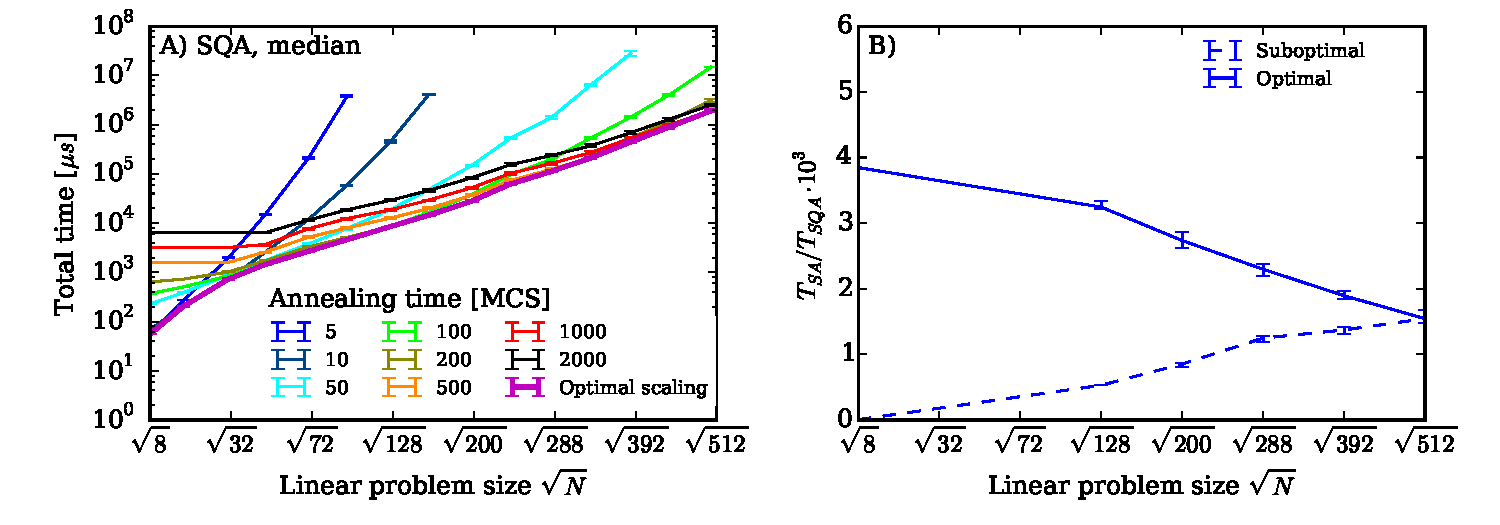
\includegraphics[width=\columnwidth]{chapters/Speedup/fig01.pdf}
\caption{{\bf Pitfalls when detecting speedup.} A) The typical (median)  time to find a ground state at least once with 99\%  probability for spin glasses with $\pm1$ couplings using SQA at constant annealing time. The lower envelope of the curves at constant $t_a$ corresponds to the total effort at an optimal size-dependent annealing time $t_a^{\rm opt}(N)$ and can be used to infer the asymptotic scaling. The initial, relatively flat slope at fixed $N$ is due to suboptimal performance at small problem sizes $N$, and should therefore not be interpreted as speedup. Annealing times are given in units of Monte Carlo steps (MCS), corresponding to one update per spin. B) The speedup of SQA over SA for two cases. If SQA is run suboptimally at small sizes by choosing a fixed large annealing time $t_a=10000$ MCS (dashed line) a speedup is feigned. This is due to suboptimal performance on small sizes and not indicative of the real asymptotic behavior when both codes are run optimally (solid line).}
\label{fig:medianfixed}
\end{figure}
%%%%%%%%%
%%%%%%%%%
\begin{figure}
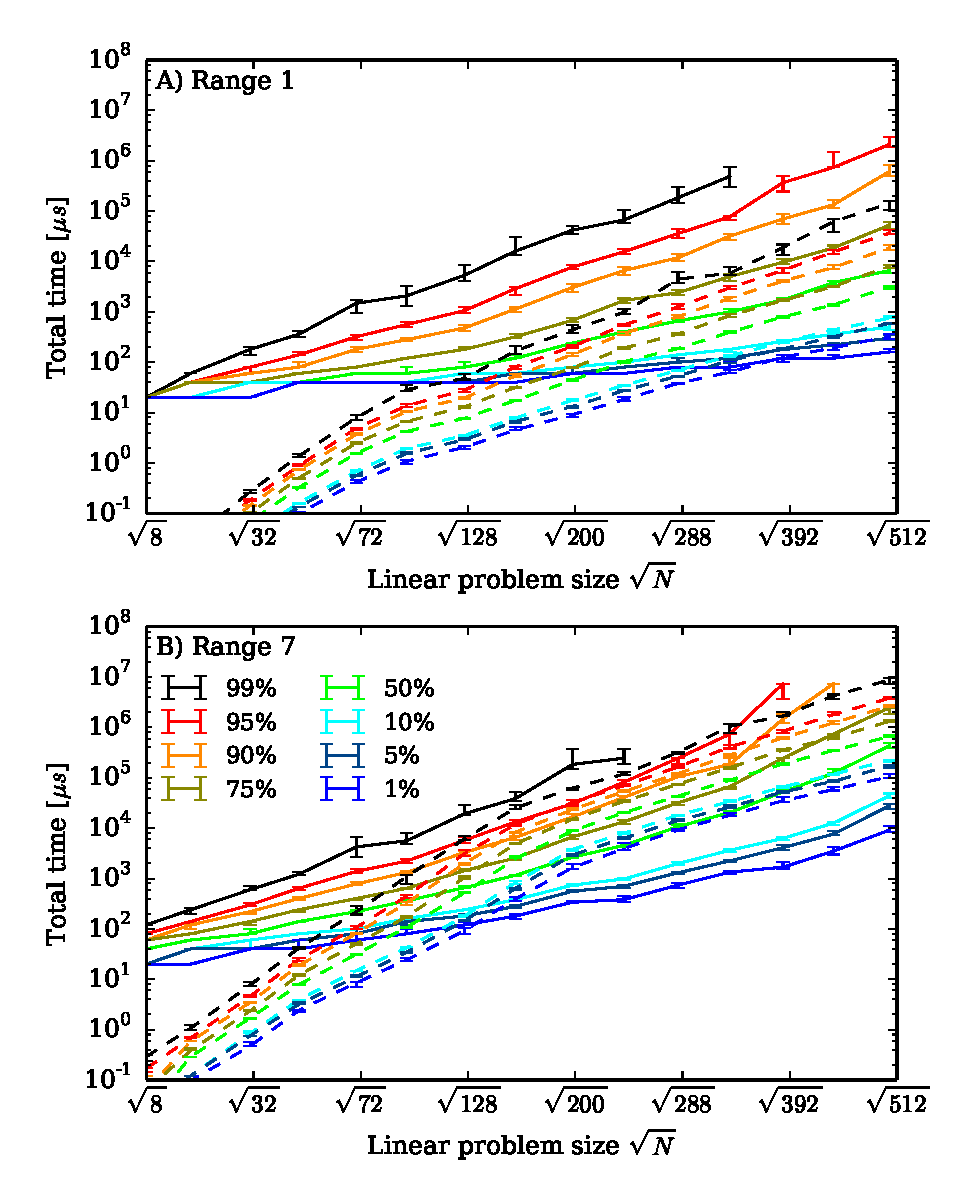
\includegraphics[width=1\columnwidth]{chapters/Speedup/fig03.pdf}
\label{fig:scalingraw7}
\caption{{\bf Scaling of time to solution for the ranges $r=1$ (panel A) and $r=7$ (panel B).} Shown is the scaling of the pure annealing time to find the ground state at least once with a probability $p=0.99$ for various quantiles of hardness, for simulated annealing (SA, dashed) and the DW2 (solid).
%The SA data was obtained by running the simulations at an optimized annealing time for each problem size. The DW2 a nnealing time of $20\mu s$ is the shortest possible.
The solid lines terminate for the highest quantiles because the DW2 did not solve the hardest instances for large problem sizes within the maximum number of repetitions (at least 32000) of the annealing we performed.
}
\label{fig:scalingraw}
\end{figure}
%%%%%%%%%
%%%%%%%%%
\begin{figure}
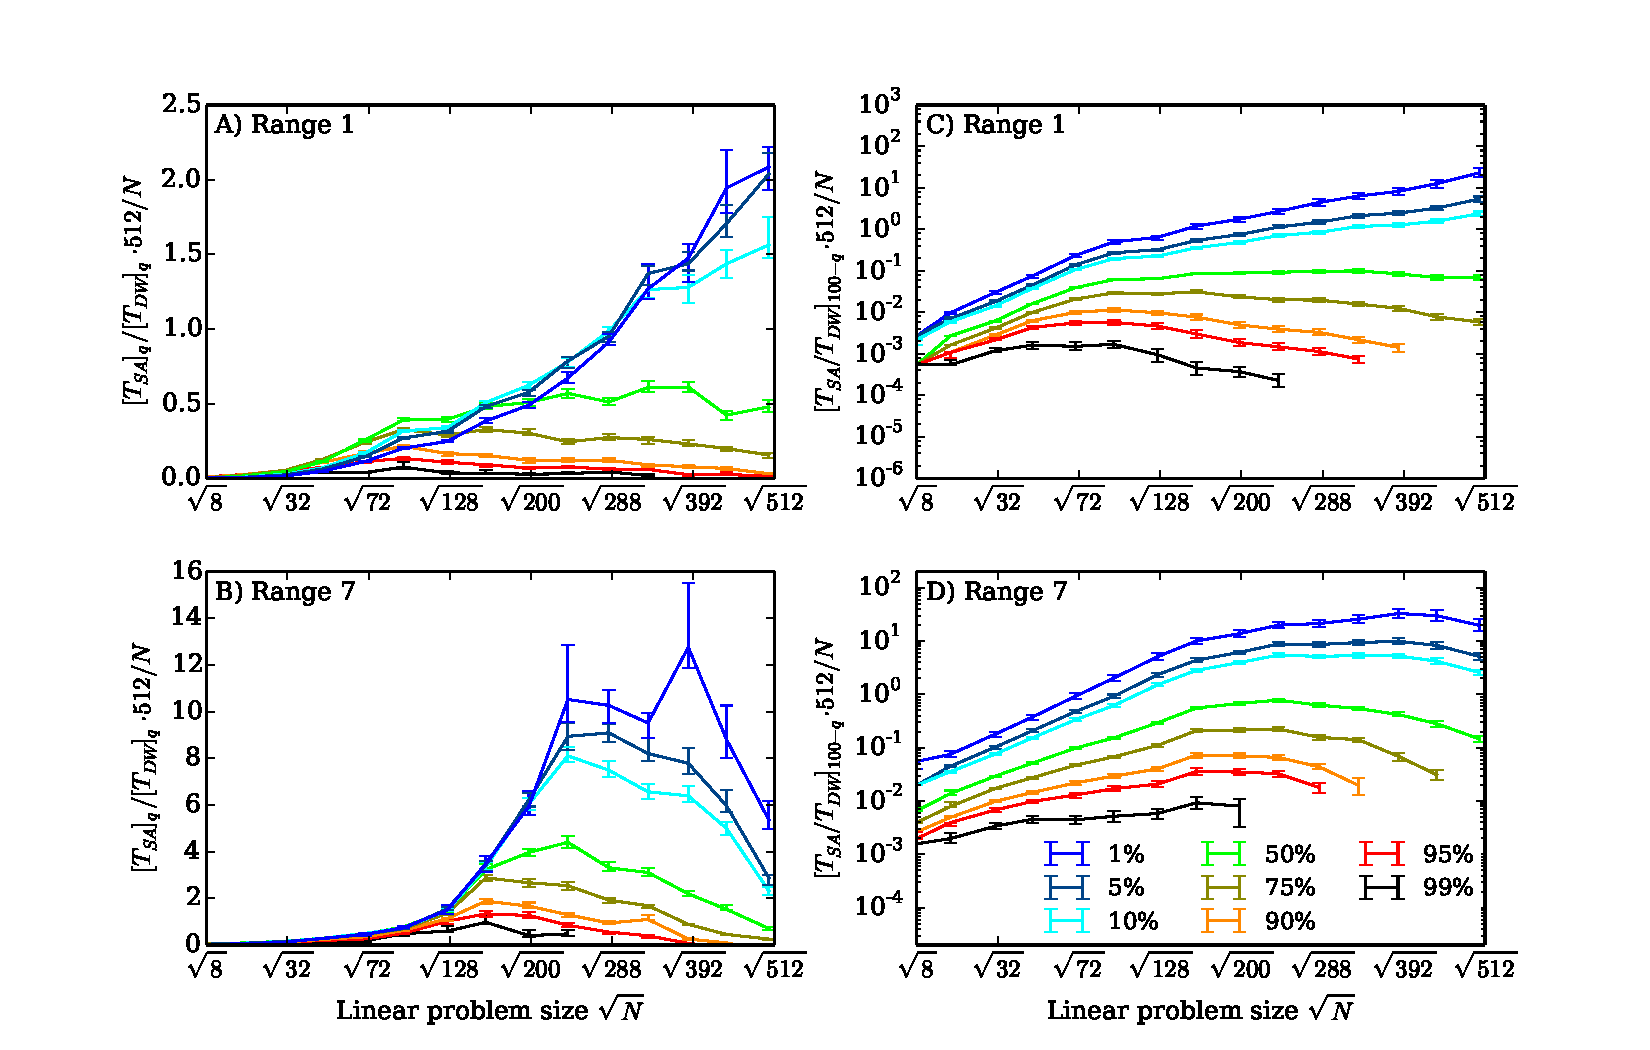
\includegraphics[width=0.95\textwidth]{chapters/Speedup/fig07.pdf}
\caption{{\bf Speedup of the DW2 compared to SA.} A) and B) for the ratio of the quantiles (RofQ), C) and D) for the quantiles of the ratio (QofR). For a random variable $X$ with distribution $p(x)$ and values in $x\in [0,\infty)$ we define, as usual, the $q$th quantile as $\int_0^{x_q} p(x) dx = q/100$, which we solve for $x_q$ and plot as a function of $\sqrt{N}$. In the QofR case we use $x_{100-q}$  so that high quantiles still correspond to instances that are hard for the DW2. We terminate the curves when the DW2 does not find the ground state for large $N$ at high percentiles. In these plots we multiplied Eqs.~\eqref{eq:S_q} and \eqref{eq:SQoR} by $512$ so that the speedup value at $N=512$ directly compares one DW2 processor against one classical CPU. An overall positive slope suggests a possible limited quantum speedup, subject to the caveats discussed in the text. A negative slope indicates that SA outperforms the DW2.
}
\label{fig:qorspeedup7}
\end{figure}
%%%%%%%%%

%%%%%%%%%
\begin{figure}
\centering
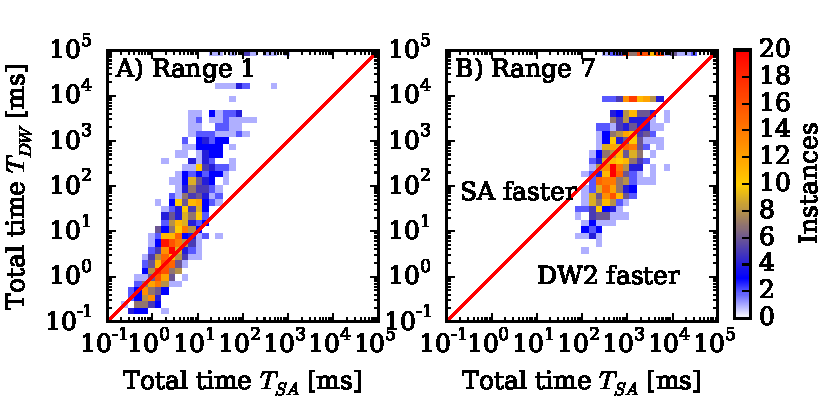
\includegraphics[width=0.95\columnwidth]{chapters/Speedup/fig06.pdf}
\label{fig:ratiosannealing}
\caption{{\bf Instance-by-instance comparison of annealing times.} Shown is a scatter plot of the pure annealing time for the DW2 compared to SA using an average over $16$ gauges (see \ref{sec:supp}) on the DW2 for A) $r=1$ and B) $r=7$.  The color scale indicates the number of instances in each square. Instances below the diagonal red line are faster on the DW2, those above are faster using SA. Instances for which the DW2 did not find the solution with 10000 repetitions per gauge are shown at the top of the frame (no such instances were found for SA).
%Panels C) and D)  show  wall-clock times using a single gauge on the DW2.
%Panels E) and F) show the wall-clock time for DW2 using $16$ gauges. $N=503$ in all cases. \red{Unless we discuss it in the text (currently not) we need to move wall-clock to SM.}
}
% \label{fig:ratiosannealing}
\end{figure}
%%%%%%%%%

%%%%%%%%%

\section{Supplementary Information}\label{sec:supp}
%More generally, a limited quantum speedup can be thought of as being the result of decohering the quantum device. Since there is no unique way to decohere a quantum device, one may arrive at different corresponding classical algorithms. \\ % I DROPPED THIS BECAUSE NORMALLY DECOHERING A DEVICE WOULD NOT GIVE A WORKING CLASSICAL ALGORITHM

% \bigskip


\subsection{Annealing methods}
\subsubsection{Quantum annealing}
The annealing schedules used in our work are shown in Figure~\ref{fig:schedule}.\\

%\input{fig9}
\begin{figure}
\centering
\includegraphics[width=0.95\textwidth]{chapters/Speedup/sfigures/sfig01.pdf}
\caption{{\bf Annealing schedules.} A) The amplitudes of the transverse fields $A_i(t)$ [decreasing, blue] and the longitudinal couplings $B(t)$ (increasing, red) as a function of time. The device temperature of $T=18$mK is indicated by the black horizontal dashed line. B) The linear annealing schedule used in simulated quantum annealing.}
\label{fig:schedule}
\end{figure}
%
%\input{fig10}

\subsubsection{Simulated annealing (SA)}
\label{sec:simulated-annealing}
During the annealing schedule we linearly increase the inverse temperature over time from an initial value of $\beta=0.1$ to a final value of $\beta=3r$.

For the case of $\pm1$ couplings ($r=1$), and  for $r=3$ we use a highly optimized multispin-coded algorithm based on Refs.~\cite{J.Stat.Phys.44.985,Comput.Phys.Commun.59.387}. This algorithm performs updates on $64$ copies in parallel, updating all at once. For the $r=7$ simulations we use a code optimized for bipartite lattices. Implementations of the simulated annealing codes are available in Ref.~\cite{sapaper}. We used the code {\tt an\_ms\_r1\_nf} for $r=1$, the code {\tt an\_ms\_r3\_nf} for $r=3$ and the code {\tt an\_ss\_ge\_nf\_bp } for $r=7$.\\


\subsubsection{Simulated quantum annealing (SQA)}
\label{sec:discr-time-quant}
The algorithm we used here is similar to that of Ref.~\cite{PhysRevB.66.094203}, but uses cluster updates along the imaginary time direction, typically with $64$ time slices. Our annealing schedule is linear, as shown in Figure~\ref{fig:schedule}B): the Ising couplings are ramped up linearly while the transverse field is ramped down linearly over time. Our SQA results for ranges $1$ and $7$, complementing Figure~2 in the main text, are shown in Figure~\ref{fig:scaling_sqa}.\\

\begin{figure}[t]
\centering
\includegraphics[width=0.95\textwidth]{chapters/Speedup/sfigures/sfig05_leftover.pdf}
\caption{{\bf Scaling of time-to-solution for SQA.} Shown is the time-to-solution A) for range $r=1$ and B) for range $r=7$.}
\label{fig:scaling_sqa}
\end{figure}

\begin{table}
  \centering
  \begin{tabular}{|c|c|c|c|}\hline
 $N\le 238$ & $N=284$, 332 & $N=385$, 439 & $N=503$ \\ \hline
 1000 & 2000 & 5000 & 10000 \\ \hline
  \end{tabular}
  \caption{{\bf Repetitions of annealing runs used on the DW2}. This table summarizes the total number of repetitions used to estimate the success probabilities on the DW2 for various system sizes.}
  \label{tab:reps}
\end{table}


All three annealing methods mentioned above are heuristic. They are not guaranteed to find the global optimum in a single annealing run, but only find it with a certain instance-dependent success probability $s\leq 1$. We determine the true ground state energy using an exact belief propagation algorithm \cite{dechter1999bucket}. We then perform at least $1000$ repetitions of the annealing for each instance, count how often the ground state has been found by comparing to the exact result, and use this to estimate the success probability $s$ for each problem instance. See Table \ref{tab:reps} for the exact number of repetitions performed on the DW2 device. \\


\subsection{The D-Wave Two Vesuvius device}
%
%\input{fig8}
\begin{figure}[h]
\centering
\includegraphics[width=0.443\textwidth]{chapters/Speedup/fig08.pdf}
\caption{\textbf{Qubits and couplers in the D-Wave Two device.} The DW2 ``Vesuvius'' chip consists of an $8\times8$ two-dimensional square lattice of eight-qubit unit cells, with open boundary conditions. The qubits are each denoted by circles, connected by programmable inductive couplers as shown by the lines between the qubits. Of the $512$ qubits of the device located at the University of Southern California used in this work, the $503$ qubits marked in green and the couplers connecting them are functional.}
\label{fig:chimeraDW2}
\end{figure}
%

The annealing schedules $A_i(t)$ and $B(t)$ used in the device are shown in figure \ref{fig:schedule}A).

\subsubsection{Our problem class}
The family of problem instances we use for our benchmarking tests employ couplings $J_{ij}$ on all edges of $N=8LL'$-vertex subgraphs of the Chimera graph of the DW2, comprising $L\times L'$ unit cells, with $L,L'\in\{1,\dots,8\}$. We set the fields $h_i=0$ since nonzero values of the fields $h_i$ destroy the spin glass phase that exists at zero field, thus making the instances easier \cite{AT}. We choose the values of the couplings $J_{ij}$ from $2r$ discrete values  $\{n/r\}$, with $n \in \{-r, -r-1, \dots, -1, 1, \dots, r-1, r\}$, and call $r$ the ``range". Thus when the range $r=1$ we only pick values $J_{ij}=\pm 1$. This choice is the least susceptible to calibration errors of the device, but the large degeneracy of the ground states in these cases makes finding a ground state somewhat easier. At the opposite end we consider $r=7$, which is the upper limit given the four bits of accuracy of the couplings in the DW2. These problem instances are harder since there are fewer degenerate minima, but they also suffer more from calibration errors in the device. We also used an annealing time of 20$\mu$s.

\subsection{Gauge averaging}\label{subsec:gauge_averaging}
Calibration inaccuracies cause the couplings $J_{ij}$ and $h_i$ that are realized in the DW2 to be slightly different from the intended and programmed values ($\sim 5\%$ variation). These calibration errors can sometimes lead to the ground states of the model realized in the device being different from the perfect model. To overcome these problems it is advantageous to perform annealing on the device with multiple encodings of a problem instance into the couplers of the device \cite{q108}. To realize these different encodings we use a gauge freedom in realizing the Ising spin glass: for each qubit we can freely define which of the two qubits states corresponds to $\sigma_i=+1$ and  $\sigma_i=-1$. More formally this corresponds to a gauge transformation that changes spins $\sigma^z_i\rightarrow  a_i\sigma^z_i$, with $a_i=\pm1$ and the couplings as $J_{ij} \rightarrow a_ia_jJ_{ij}$ and $h_i\rightarrow a_ih_i$. The simulations are invariant under such a gauge transformation, but (due to calibration errors which break the gauge symmetry) the results returned by the DW2 are not.

If the success probability of one annealing run is denoted by $s$, then the probability of failing to find the ground state after $R$ independent repetitions (annealing runs) each having success probability $s$ is $(1-s)^R$, and the total success probability of finding the ground state at least once in $R$ repetitions is
\begin{equation}
 P=1-(1-s)^R .
 \label{eq:oneg}
 \end{equation}
Thus the number of repetitions needed to find the ground state at least once with probability $P$ is found by isolating $R$ in Eq.~\eqref{eq:oneg}.

Following \cite{q108}, after splitting these repetitions into $R/G$ repetitions for each of $G$ gauge choices with success probabilities $s_g$, the total success probability becomes
 \begin{equation}
 P^{(G)} = 1-\prod_{g=1}^G(1-s_g)^{R/G}.
 \label{eq:manyq}
 \end{equation}
If we use the geometric mean of the failure probabilities of the individual gauges to define
 \begin{equation}
\overline{s} = 1-\prod_{g=1}^G(1-s_g)^{1/G},
 \end{equation}
then Eq.~\eqref{eq:manyq} can be written in the same form as Eq.~\eqref{eq:oneg}:
\begin{equation}
 P^{(G)}=1-(1-\overline{s})^R.
 \label{eq:onegav}
 \end{equation}
We thus use the geometric mean $\overline{s}$ in our scaling analysis.\\

\begin{figure}
%\centering
\subfloat[]{\includegraphics[width=0.49\columnwidth]{chapters/Speedup/sfigures/sfig08.pdf}\label{fig:wall-clock1}}
\subfloat[]{\includegraphics[width=0.49\columnwidth]{chapters/Speedup/fig05.pdf}\label{fig:wall-clock2}}
% \end{figure}
%\includegraphics[width=0.5\textwidth]{sfigures/sfig08.pdf}
\caption{{\bf Comparing wall-clock times.} A comparison of the wall-clock time to find the solution with probability $p=0.99$ for SA running on a single CPU (dashed lines) compared to the DW2 [solid lines] using a single gauge choice in the left column and $16$ gauges in the right column. A) for range $r=1$, B) for range $r=3$, C) for range $r=7$. Shown are curves from the median ($50$th quantile) to the $99$th quantile. The large constant programming overhead of the DW2 masks the exponential increase of time-to-solution that is obvious in the plots of pure annealing time.}
\label{fig:wall-clock}
\end{figure}


\subsection{Annealing and wall-clock times}
\label{sec:wall-clock-annealing-class}
A complementary distinction is that between {wall-clock time}, denoting the full time-to-solution, and the {pure annealing time}. Wall-clock time is the total time to find a solution and is the relevant quantity when one is interested in the performance of a device for applications and has been used in Ref. \cite{McGeoch}. It includes the setup, cooling, annealing and readout times on the DW2, and the setup, annealing and measurement time for the classical annealing codes.
The pure annealing time for $R$ repetitions is straightforwardly defined as
\begin{equation}
t_{\rm anneal}=Rt_a,
\end{equation}
where $t_a$ the time used for a single annealing run. It is the relevant quantity when one is interested in the intrinsic physics of the annealing processes and in scaling to larger problem sizes on future devices.

In order to measure wallclock times on the DW2 we have performed tests with varying numbers of repetitions $R$ and performed a linear regression analysis to fit the total wall clock time for each problem size to the form $t_p(N)+Rt_r(N)$, where $t_p(N)$ is the total preprocessing time and $t_r(N)$ is the total run time per repetition for an $N$-spin problem. The values of $t_p$ and $t_r$ are summarized in Table \ref{tab:dw2times}. With these numbers we obtain the total wall clock time for $R$ annealing runs split over $G$ gauges (with $R/G$ annealing runs each) as
\begin{equation}
t_{\rm total}(N)=Gt_p(N)+Rt_r(N) .\\
\label{eq:wc}
\end{equation}


\begin{table}
\centering
\begin{tabular}{|c|c|c|}
\hline
$N$ & $t_p$ [ms] & $t_r$ [$\mu$s] \\
\hline
8 & $14.7 \pm 0.3$ & $51.0 \pm 0.2$ \\
16 & $14.8 \pm 0.3$ & $53.0 \pm 0.2$ \\
31 & $14.8 \pm 0.3$ & $57.9 \pm 0.2$ \\
47 & $14.9 \pm 0.4$ & $60.6 \pm 0.2$ \\
70 & $15.0 \pm 0.4$ & $64.5 \pm 0.2$ \\
94 & $15.2 \pm 0.3$ & $68.3 \pm 0.2$ \\
126 & $15.6 \pm 0.2$ & $73.1 \pm 0.2$ \\
158 & $15.5 \pm 0.2$ & $78.0 \pm 0.2$ \\
198 & $15.5 \pm 0.2$ & $80.8  \pm 0.2$ \\
238 & $15.7 \pm 0.2$ & $83.5 \pm 0.2$ \\
284 & $15.8 \pm 0.2$ & $83.6 \pm 0.1$ \\
332 & $16.0 \pm 0.3$ & $87.1 \pm 0.2$ \\
385 & $16.6 \pm 1.0$ & $87.1 \pm 0.6$ \\
439 & $16.6 \pm 0.1$ & $90.4 \pm 0.1$ \\
503 & $16.6 \pm 0.2$ & $90.5 \pm 0.1$ \\
\hline
\end{tabular}
\caption{{\bf Wallclock times on the DW2}. Listed are measured programming times $t_p$ and annealing plus readout times $t_r$ (for a pure annealing time of $20\mu$s) on the DW2 for various problem sizes.}
\label{tab:dw2times}
\end{table}



%\subsection{Classical algorithms}
%\label{sec:classical-programs}


To calculate pure annealing times for the simulated annealer we  determine the total effort in units of Monte Carlo updates (attempted spin flips), and then convert to time by dividing by the number of updates that the codes can perform per second \cite{sapaper}. Our classical reference CPU is an $8$-core Intel Xeon E5-2670 CPU, which was introduced around the same time as the DW2.

To obtain wall-clock times we measure the actual time needed to perform a simulation on the same  Intel Xeon E5-2670 CPU. Since the multi-spin codes perform at $64$ repetitions in parallel, we always make at least $1024$ repetitions when running 16 threads on $8$ cores. This causes the initially flatter scaling in wall-clock times as compared to pure annealing times (Figure~\ref{fig:wall-clock}). The measured initialization time includes all preparations needed for the algorithm to run, and the spin flip rate was computed for the 99\% quantile for 503 qubits. For smaller system sizes or lower quantiles, the spin flip rate is lower since the problems are not hard enough to benefit from parallelization over several cores.\\

While not as interesting from a complexity theory point of view, it is instructive to also compare wall-clock times for the above benchmarks, as we do in
%Figures~\ref{fig:wall-clock1}~and~\ref{fig:wall-clock2}.
Figure~\ref{fig:wall-clock}. We observe that the DW2 performs similarly to SA run on a single classical CPU, for sufficiently large problem sizes and at high range values. Note that the large constant programming overhead of the DW2 masks the exponential increase of time-to-solution that is obvious in the plots of pure annealing time.



%\begin{figure}
%\caption{{\bf Comparing wall-clock times} A comparison of the wall-clock time to find the solution with probability $p=0.99$ for SA running on a single CPU (dashed lines) compared to the DW2 (solid lines) using $16$ gauges. A) for range $r=1$,  B) for range $r=3$ and C) for range $r=7$. Shown are curves from the median ($50$th quantile) to the $99$th quantile. The large constant programming overhead of the DW2 masks the exponential increase of time-to-solution that is obvious in the plots of pure annealing time. Results for a single gauge are shown in the Supplementary Material.}
%\centering
%\includegraphics[width=0.5\textwidth]{fig05.pdf}
%\label{fig:wall-clock2}
%\end{figure}


Considering the wall-clock times, the advantage of the DW2 seen in Figure~4 A-B (in the main text) for some instances tends to disappear, since it is penalized by the need for programming the device with multiple different gauge choices. Figure~\ref{fig:ratiosannealingSI}A-F shows that for one gauge choice there are some instances, for $r=7$, where the DW2 is faster, but many instances where it never finds a solution. Using $16$ gauges the DW2 finds the solution in most cases, but is always slower than the classical annealer on a classical CPU for $r=1$, as can be seen in Figure~\ref{fig:ratiosannealingSI}A and D. For $r=7$ the DW2 is sometimes faster than a single classical CPU. Overall, the performance of the DW2 is better for $r=7$ than for $r=1$, and comparable to SA only when just the pure annealing time is considered. The difference compared to the results of Ref. \cite{McGeoch} is due to the use of optimized classical codes using a full CPU in our comparison, as opposed to the use of generic optimization codes using only a single CPU core in Ref. \cite{McGeoch}.\\


\begin{figure}
\centering
\includegraphics[width=0.7\textwidth]{chapters/Speedup/sfigures/sfig06_leftover.pdf}
\caption{{\bf Instance-by-instance comparison.} Shown is a scatter plot of the total time for the DW2 device (DW) compared to a simulated classical annealer (SA) A and D) for $r=1$, B and E) for $r=3$, and C and F) for $r=7$.
A, B and C) wall-clock time using a single gauge on the DW2, and, D, E and F)  wall-clock time using $16$ gauges on the DW2.  The color scale indicates the number of instances in each square. Instances below the diagonal red line are faster on the DW2, those above are faster classically.
Instances for which the DW2 device did not find the solution are shown at the top. SA found a solution for every instance of this benchmark.}
\label{fig:ratiosannealingSI}
\end{figure}



\subsection{Optimal annealing times}
\label{sec:scaling-optimality}
As discussed in the main text we need to determine the optimal annealing time $t_a^{\textrm{opt}}$ for every problem size $N$ in order to make meaningful extrapolations of the time to find a solution. To determine $t_a^{\textrm{opt}}$ we perform annealing runs at different annealing times $t_a$, determine the success probabilities $s(t_a)$ of 1000 instances, and from them the required number of repetitions $R(t_a)$ to find the ground state with a probability of 99\%. That is, we solve Eq.~\eqref{eq:onegav} for $R$ while setting $P^{(G)} = 0.99$:
%
\begin{equation}
R(t_a) = \left\lceil\frac{\log[1-P^{(G)}]}{\log[1-\bar{s}(t_a)]}\right\rceil\ .
\label{eq:R}
\end{equation}
%
The total effort $R(t_a)t_a$ diverges for $t_a\rightarrow 0$ and $t_a\rightarrow\infty$ and has a minimum at an optimal annealing time $t_a^{\textrm{opt}}$. The reason is that for short $t_a$ the success probability $\bar{s}(t_a)$ goes to zero, which leads to a diverging total effort, while for large $t_a$ the time also grows since one always needs to perform at least one annealing run and the total effort is thus bounded from below by $t_a$.

\begin{figure}[t]
\includegraphics[width=0.95\textwidth]{chapters/Speedup/fig10.pdf}
%\subfigure{\includegraphics[width=0.9\columnwidth]{ssfig03.pdf}}
\caption{{\bf Optimal annealing times for the simulated annealer and for the D-Wave device.} Shown is the total effort $R(t_a)t_a$ as a function of annealing time $t_a$ for various quantiles of problems with $r=1$ and $r=7$. A) and B) SA, where the minimum of the total effort determines the optimal annealing time $t_a^{\textrm{opt}}$.  C) and D) DW2, where we find a monotonically increasing total effort, meaning that the optimal time $t_a^{\textrm{opt}}$ is always shorter than the minimal annealing time of $20\mu$s.}
\label{fig:satopt}
\end{figure}
%


In Figure~\ref{fig:satopt} (left) we plot various quantiles of the total effort $R(t_a)t_a$ for the simulated annealer as a function of $t_a$ to determine the  optimal annealing time $t_a^{\textrm{opt}}$. For the DW2 we find, as shown in Figure~\ref{fig:satopt} (right) that the minimal annealing time of  $20\mu s$  is always longer than the optimal time and we thus always use the device in a suboptimal mode. As a consequence the scaling of time-to-solution is underestimated, as explained in detail in the main text.

While one can in principle look for an optimal annealing time for each individual problem instance, our approach is to instead determine an averaged optimal annealing time $t_a^{\textrm{opt}}(N)$ for each problem size $N$ by annealing many instances at various annealing times $t_a$, and then use these for all future problems of that size.\\


\subsection{Resource usage and speedup from parallelism}

In the main text we saw that in order to avoid mistaking a parallel speedup for a quantum speedup we need to scale hardware resources  (computational gates and memory) in the same way for the devices we compare, and employ these resources optimally. These considerations are not universal but need to be carefully applied for each comparison of a quantum algorithm and device to a classical one. Here we provide several independent derivations that lead us to the same conclusion.

Recall that in the main text we argued that the {\em quantum} part of speedup is estimated by comparing the times required by two devices with the same hardware scaling, giving
%
\begin{equation}
S(N) = \frac{T_{\textrm{C}}(N)}{T_{\textrm{DW}}(N)} \propto  \frac{T_{\textrm{SA}}(N)}{T_{\textrm{DW}}(N)} \frac{1}{N}\ ,
\label{eq:parallelspeedup1SI}
\end{equation}
%
which is Eq.~(3) of the main text. The factor $1/N$ in the speedup calculation discounts for the intrinsic \emph{parallel speedup} of the analog device whose hardware resources scale as $N$, compared to a fixed size classical device used for the timings.

\subsubsection{Derivation assuming fixed computational resources}
In the consideration of how to disentangle parallel and quantum speedup it may seem more natural to assume fixed computational resources of a given device. We will show that this leads to the same scaling as Eq.~\eqref{eq:parallelspeedup1SI}.

We might be tempted to define the speedup in this case as
$S(N) = \frac{{T_{\textrm{SA}}(N)}}{{T_{\textrm{DW}}(N)}}$.
However, in this manner only a fraction $N/512$ of the qubits are used while the classical code uses the available CPU fully, independently of problem size. This suboptimal use of the DW2 may again be incorrectly interpreted as speedup. The same issue would appear when comparing a classical analog annealer against a classical simulated annealer.

 As in the discussion of optimal annealing times above, we need to ensure an optimal implementation to correctly assess speedup. For the DW2 (or a similarly constructed classical analog annealer) this means that one should always attempt to make use of the entire device: we should perform as many annealing runs in parallel as possible.
Let us denote the machine size by $M$ (e.g., $M=512$ in the DW2 case). With this we define a new, optimized, annealing time
\begin{equation}
T^{\rm opt}_{\textrm{DW}}(N) = T_{\textrm{DW}}(N) \frac{1}{\lfloor M/N\rfloor} ,
\label{eq:T^opt_DW}
\end{equation}
and the speedup in our case is then
\begin{equation}
S(N) = \frac{T_{\textrm{SA}}(N)}{T^{\rm opt}_{\textrm{DW}}(N)} =  \frac{T_{\textrm{SA}}(N)}{T_{\textrm{DW}}(N)} \left\lfloor\frac{M}{N}\right\rfloor.
\label{eq:parallelspeedup2}
\end{equation}

Omitting the floor function ($\lfloor \; \rfloor$), which only gives subdominant corrections in the limit $M\rightarrow\infty$ we recover Eq.~\eqref{eq:parallelspeedup1SI}.


\subsubsection{Derivation from the scaling of the annealing time.}
The conclusion that the speedup function includes a factor proportional to $1/N$ is validated from yet another perspective, that focuses on the annealing time. Instead of embedding $C\equiv \lfloor{M}/{N}\rfloor$ different instances in parallel, we can embed $C$ replicas of a given instance.
Each replica $r$ (where $r\in\{1,\dots,C\}$) results in a guess $E_{r,i}$ of the ground state energy for the $i$th run, and we can take $E_i = \min_r E_{r,i}$ as the proposed solution for that run.
If the replicas are independent and each has equal probability $s$ of finding the ground state, then
using $C$ replicas the probability that at least one will find the ground state is $s' = 1-(1-s)^C$, which is also the probability that $E_i$ is the ground state energy for the $i$th run. Repeating the argument leading to Eq.~\eqref{eq:R}, the number of repetitions required to find the ground state at least once with probability $p$ is then:
\begin{equation}
  R' =
  \left\lceil
    \frac{\log (1-p)}{\log(1 - s')}
    \right\rceil
    = \left\lceil
    \frac{\log (1-p)}{C\log(1 - s)}\right\rceil ,
%    =\frac{R}{C} .
\end{equation}
while $R = \left\lceil\frac{\log (1-p)}{\log(1 - s)}\right\rceil$. It is easy to show that $R'-1\leq R/C \leq R'$.
Focusing on the pure annealing time we have $T^{\rm opt}_{\textrm{DW}}(N) = t_a R'$ and $T_{\textrm{DW}}(N) = t_a R$, which yields Eq.~\eqref{eq:T^opt_DW} in the limit of large $R$.\\

\subsection{Arguments for and against a speedup on the DW2}

Let us consider in more detail the speedup results discussed in the main text and above. We have argued that the apparent limited quantum speedup seen in the $r=1$ results of Figure~3 in the main text must be treated with care due to the suboptimal annealing time. It might then be tempting to argue that, strictly speaking, the comparison with suboptimal-time instances cannot be used for claiming a slowdown either, i.e., that we simply cannot infer how the DW2 will behave for optimal-time instances by basing the analysis on suboptimal times only.

However, let us make the assumption that, along with the total time, the optimal annealing time $t_a^{\textrm{opt}}(N)$ also grows with problem size $N$. This assumption is supported by the SA and SQA data shown in Figure~1 in the main text and Figure~\ref{fig:leftover02}, and is plausible as long as the growing annealing time does not become counterproductive due to coupling to the thermal bath \cite{PhysRevLett.95.250503}. By definition,  $T_{\textrm{DW}}(N,t_a^{\textrm{opt}}(N)) \leq T_{\textrm{DW}}(N,t_a)$, where we have added the explicit dependence on the annealing time, and $t_a$ is a fixed annealing time. Thus
\begin{align}
S(N) &= \frac{T_{\textrm{C}}(N)}{T_{\textrm{DW}}(N,t_a)}\frac{1}{N}  \\
&\leq \frac{T_{\textrm{C}}(N)}{T_{\textrm{DW}}(N,t_a^{\textrm{opt}}(N))}\frac{1}{N} = S^{\textrm{opt}}(N) \notag.
\end{align}
Under our assumption, $t_a^{\textrm{opt}}(N) < t_a $ for small $N$, but for sufficiently large $N$ the optimal annealing time grows so that $t_a^{\textrm{opt}}(N) \geq t_a$. Thus there must be a problem size $N^*$ at which $t_a^{\textrm{opt}}(N^*) = t_a$, and hence at this special problem size we also have $S(N^*) = S^{\textrm{opt}}(N^*)$. However, the minimal annealing time of $20\mu s$ is longer than the optimal time for all problem sizes (see Figure~\ref{fig:satopt}), i.e., $N^*>503$ in our case. Therefore, if $S(N)$ is a decreasing function of $N$ for sufficiently large $N$, as we indeed observe in all our RofQ results (recall Figure 3A and B in the main text), then since $S^{\textrm{opt}}(N) \geq S(N)$ {and} $S(N^*) = S^{\textrm{opt}}(N^*)$, it follows that $S^{\textrm{opt}}(N)$ too must be a decreasing function for a range of $N$ values, at least until $N^*$. This shows that the slowdown conclusion holds also for the case of optimal annealing times.

For the instance-by-instance comparison (QofR), no such conclusion can be drawn for the subset of instances (at $r=1$) corresponding to the high quantiles where $S_q^{\textrm{QofR}}(N)$ is an {increasing} function of $N$. This limited quantum speedup may or may not persist for larger problem sizes or if optimal annealing times are used. \\

\subsection{Additional Discussion}\label{subsec:additional}

In this work we have discussed challenges in properly defining and assessing quantum speedup, and used comparisons between a DW2 and simulated classical and quantum annealing to illustrate these challenges. \emph{Strong} or \emph{provable} quantum speedup, implying speedup of a quantum algorithm or device over \emph{any} classical algorithm, is an elusive goal in most cases and one thus usually defines \emph{quantum speedup} as a speedup compared to the best available classical algorithm. We have introduced the notion of \emph{limited quantum speedup}, referring to a more restricted comparison to `corresponding' classical algorithms solving the same task, such as a quantum annealer compared to a classical annealing algorithm.

Quantum speedup is most easily defined and detected in the case of an exponential speedup, where the details of the quantum or classical hardware do not matter since they only contribute subdominant polynomial factors. In the case of an unknown or a polynomial quantum speedup one must be careful to fairly compare the classical and quantum devices, and, in particular, to scale hardware resources in the same manner. Otherwise \emph{parallel speedup} might be mistaken for (or hide) quantum speedup.

An experimental determination of quantum speedup suffers from the problem that all measurements are limited to finite problem sizes $N$, while we are most interested in the asymptotic behavior for large $N$. To arrive at a reliable extrapolation it is advantageous to focus the scaling analysis on the part of the execution time that becomes dominant for large problem sizes $N$, which in our example is the pure annealing time, and not the total wall-clock time. For each problem size we furthermore need to ensure that neither the quantum device nor the classical algorithm are run suboptimally, since this might hide or fake quantum speedup.

If the time to solution depends not only on the problem size $N$ but also on the specific problem instance, then one needs to carefully choose the relevant quantity to benchmark. We argued that in order to judge the performance over many possible inputs of a randomized benchmark test, one needs to study the high quantiles, and define speedup by considering the ratio of the quantiles of time to solution. If, on the other hand, one is interested in finding out whether there is a speedup for some subset of problem instances, then one can instead perform an instance-by-instance comparison by focusing on the quantiles of the ratio of time to solution.

We chose to focus here on the benchmark problem of random zero-field Ising problems parametrized by the range of couplings.
We did not find evidence of limited quantum speedup for the DW2 relative to simulated annealing in our particular benchmark set when we considered the ratio of quantiles of time to solution, which is the relevant quantity for the performance of a device as an optimizer. We note that random spin glass problems, while an interesting and important physics problem, may not be the most relevant benchmark for practical applications, for which other benchmarks may have to be studied.

When we focus on subsets of problem instances in an instance-by-instance comparison, we observe a possibility for a limited quantum speedup for a fraction of the instances. (The fact that some problems are solved faster on classical hardware and some on the DW2 raises the possibility of a hybrid approach that benefits by solving a problem instance using both, and then selecting the best solution found.) However, since the DW2 runs at a suboptimal annealing time for most of the corresponding problem instances, the observed speedup may be an artifact of attempting to solve the smaller problem sizes using  an excessively long annealing time. This difficulty can only be overcome by fixing the issue of suboptimal annealing times, e.g., by finding problem classes for which the annealing time is demonstrably already optimal.
Alternatively, other problem classes might exhibit a speedup. For example, it is possible that a randomized benchmark with a tunable ``hardness knob", such as the clause density in the MAX-2SAT problem \cite{MAX2SAT}, will allow for a more fine-tuned exploration of the performance potential of a quantum annealer than a purely randomized benchmark such as we have used here. It was also proposed that embedding 3D spin-glass problems into the Chimera graph, with a finite critical temperature, might yield problem classes that are better suited as benchmarks for quantum annealing \cite{2014Katzgraber}.

\subsection{Additional scaling data: range $3$}
\label{sec:scaling-all-ranges}

\begin{figure}[t]
\centering
\includegraphics[width=0.95\textwidth]{chapters/Speedup/sfigures/sfig04.pdf}
\caption{{\bf Scaling of time-to-solution for $r=3$.} Shown is the scaling for the time to find the ground state with a probability of 99\% for various quantiles of hardness for A) the simulated annealer, B) the simulated quantum annealer, and C) the DW2 device.}
\label{fig:scalingraw3}
\end{figure}

\begin{figure}[t]
%\centering
\subfloat[]{\includegraphics[width=0.49\textwidth]{chapters/Speedup/sfigures/sfig05.pdf}}
\subfloat[]{\includegraphics[width=0.49\textwidth]{chapters/Speedup/sfigures/sfig07.pdf}}
\caption{{\bf Speedup for the DW2 device compared to SA for instances with $r=3$.} $16$ gauges were used. Left: the ratio of quantiles (RofQ). Right:  quantiles of the ratio (QofR).  The results are intermediate between the $r=1$ and $r=7$ results as discussed in the text.}
\label{fig:roq-qofr-speedup3}
\end{figure}

Scaling plots for range $3$ instances, requiring $3$ bits of precision in the couplings, are shown in Figure~\ref{fig:scalingraw3}, complementing Figure~2 in the main text. Figure~\ref{fig:roq-qofr-speedup3} (left) displays the ratio of quantiles and, like Figure~3 in the main text, does not exhibit a limited quantum speedup.
Figure~\ref{fig:roq-qofr-speedup3} (right) displays the results for the quantiles of ratio of time-to-solution. The results are intermediate between those seen in Figure~3 in the main text for $r=1,7$, namely, while for $r=1$ there appears to be a limited quantum speedup (relative to SA) for the higher quantiles, this speedup disappears for $r=7$; for $r=3$ we observe a flattening of the speedup curves starting at the $10$th percentile, while the higher percentiles bend down. The same suboptimality remarks discussed in this context in the main text apply. We have obtained similar results (not shown) for ranges $r=2,4,5,6$ and for instances including random longitudinal fields.

Figure \ref{fig:ratiosannealingSI3} shows the instance-by-instance comparisons for the pure annealing time. The conclusions are very similar to those obtained based on Figure~4 in the main text using the $r=1,7$ data. \\

\begin{figure}
\centering
\includegraphics[width=0.7\textwidth]{chapters/Speedup/sfigures/sfig06.pdf}
\caption{{\bf Instance-by-instance comparison for $r=3$.} Comparison between time-to-solution for SA and DW2 using pure annealing times and using $16$ gauges. }
\label{fig:ratiosannealingSI3}
\end{figure}


\begin{figure}
\centering
\includegraphics[width=0.7\textwidth]{chapters/Speedup/sfigures/sfig02_leftover.pdf}
\caption{{\bf Optimal annealing times for SA.} Shown is the time-to-solution for various quantiles as a function of annealing time (Monte Carlo steps) for SA range $r=1$. This supplements Figure~1 in the main text.}
\label{fig:leftover02}
\end{figure}


\clearpage

%%%%%%%%%
% \bibliographystyle{Science}
% \bibliography{speedup_refs}
%%%%%%%%%



% \end{document}

% \end{document}
